%% ===========================================================================
%% 硕士学位论文 全文草稿
%% 题目：青翘、乌药、黄连、虎杖、赤芍、败酱草大鼠入血成分分析
%%       及网络药理学研究
%% 版本：v2（全章节完整版）
%% 编译：XeLaTeX → BibTeX → XeLaTeX × 2
%% 参考文献格式：GB/T 7714-2015
%% ===========================================================================

\documentclass[12pt,a4paper,UTF8,openany]{ctexbook}

%% ===== 页面设置 =====
\usepackage[
  top=3.0cm, bottom=2.5cm,
  left=3.0cm, right=2.5cm,
  headheight=1.5cm
]{geometry}

%% ===== 字体与编码 =====
\usepackage{fontspec}
\usepackage{xunicode}

%% ===== 行距与排版 =====
\usepackage{setspace}
\usepackage{microtype}
\setstretch{1.5}

%% ===== 图表 =====
\usepackage{graphicx}
\usepackage{float}
\usepackage{caption}
\usepackage{subcaption}
\usepackage{booktabs}
\usepackage{array}
\usepackage{longtable}
\usepackage{tabularx}
\usepackage{multirow}
\usepackage{xcolor}

%% ===== 数学 =====
\usepackage{amsmath}
\usepackage{amssymb}

%% ===== 特殊环境 =====
\usepackage{mdframed}
\usepackage{tcolorbox}
\tcbuselibrary{skins,breakable}

%% ===== 引用与超链接 =====
\usepackage[numbers,super,square,sort&compress]{natbib}
\usepackage[
  colorlinks=true,
  linkcolor=blue!70!black,
  citecolor=blue!70!black,
  urlcolor=blue!70!black,
  bookmarks=true,
  bookmarksnumbered=true,
  pdfauthor={K-Dense Web},
  pdftitle={青翘乌药黄连虎杖赤芍败酱草大鼠入血成分分析及网络药理学研究},
  pdfsubject={中药血清药物化学 硕士学位论文},
  pdfkeywords={血清药物化学, UPLC-MS/MS, 入血成分, 网络药理学, 中药配伍}
]{hyperref}

%% ===== 页眉页脚 =====
\usepackage{fancyhdr}
\pagestyle{fancy}
\fancyhf{}
\fancyhead[L]{\small\kaishu 硕士学位论文}
\fancyhead[R]{\small\kaishu \leftmark}
\fancyfoot[C]{\thepage}
\renewcommand{\headrulewidth}{0.4pt}
\renewcommand{\footrulewidth}{0pt}
\fancypagestyle{plain}{
  \fancyhf{}
  \fancyfoot[C]{\thepage}
  \renewcommand{\headrulewidth}{0pt}
}

%% ===== 章节格式 =====
\ctexset{
  chapter={
    format=\zihao{-2}\bfseries\centering,
    name={第,章},
    number=\chinese{chapter},
    beforeskip=20pt,
    afterskip=20pt,
  },
  section={
    format=\zihao{-3}\bfseries\raggedright,
    numberformat=\bfseries,
  },
  subsection={
    format=\zihao{4}\bfseries\raggedright,
  },
  subsubsection={
    format=\zihao{-4}\bfseries\raggedright,
  },
}

%% ===== 图注格式 =====
\captionsetup{
  font={small},
  labelfont={bf},
  labelsep=quad,
  justification=justified,
}

%% ===== 占位符框 =====
\newtcolorbox{placeholder}[1][]{
  colback=yellow!10!white,
  colframe=orange!80!black,
  fonttitle=\bfseries\small,
  title={\faIcon{edit}~数据填写区域 | DATA ENTRY AREA},
  breakable,
  #1
}

%% 简化版占位符（不使用fontawesome）
\newenvironment{databox}[1]{
  \begin{tcolorbox}[
    colback=orange!5!white,
    colframe=orange!60!black,
    title={\textbf{【待填入数据】} #1},
    fonttitle=\small\bfseries,
    breakable
  ]
}{
  \end{tcolorbox}
}

%% ===== 自定义命令 =====
\newcommand{\compoundname}[1]{\textbf{#1}}
\newcommand{\herbname}[1]{\textit{#1}}
\newcommand{\keyterm}[1]{\textbf{#1}}
\newcommand{\placeholder}[1]{%
  \begin{center}
    \fcolorbox{orange!80!black}{orange!8!white}{%
      \parbox{0.9\textwidth}{\centering\small\bfseries\color{orange!60!black}
        〔待填入：#1〕}%
    }
  \end{center}
}

%% ===========================================================================
%% 文档主体
%% ===========================================================================
\begin{document}

%% ===== 封面 =====
\begin{titlepage}
\centering
\vspace*{1.5cm}

{\zihao{2}\bfseries\kaishu 硕士学位论文}

\vspace{1cm}
\rule{\textwidth}{1pt}
\vspace{0.5cm}

{\zihao{-2}\bfseries\heiti
青翘、乌药、黄连、虎杖、赤芍、败酱草\\[0.5em]
大鼠入血成分分析\\[0.5em]
及网络药理学研究
}

\vspace{0.3cm}
{\zihao{3}\kaishu
Serum Pharmacochemistry of Six Traditional Chinese Medicines\\
\textit{(Forsythiae Fructus, Linderae Radix, Coptidis Rhizoma,}\\
\textit{Polygoni Cuspidati Rhizoma et Radix, Paeoniae Radix Rubra,}\\
\textit{Patriniae Herba)} and Network Pharmacology Study in Rats
}

\vspace{0.5cm}
\rule{\textwidth}{0.5pt}

\vspace{1cm}

\begin{figure}[H]
\centering
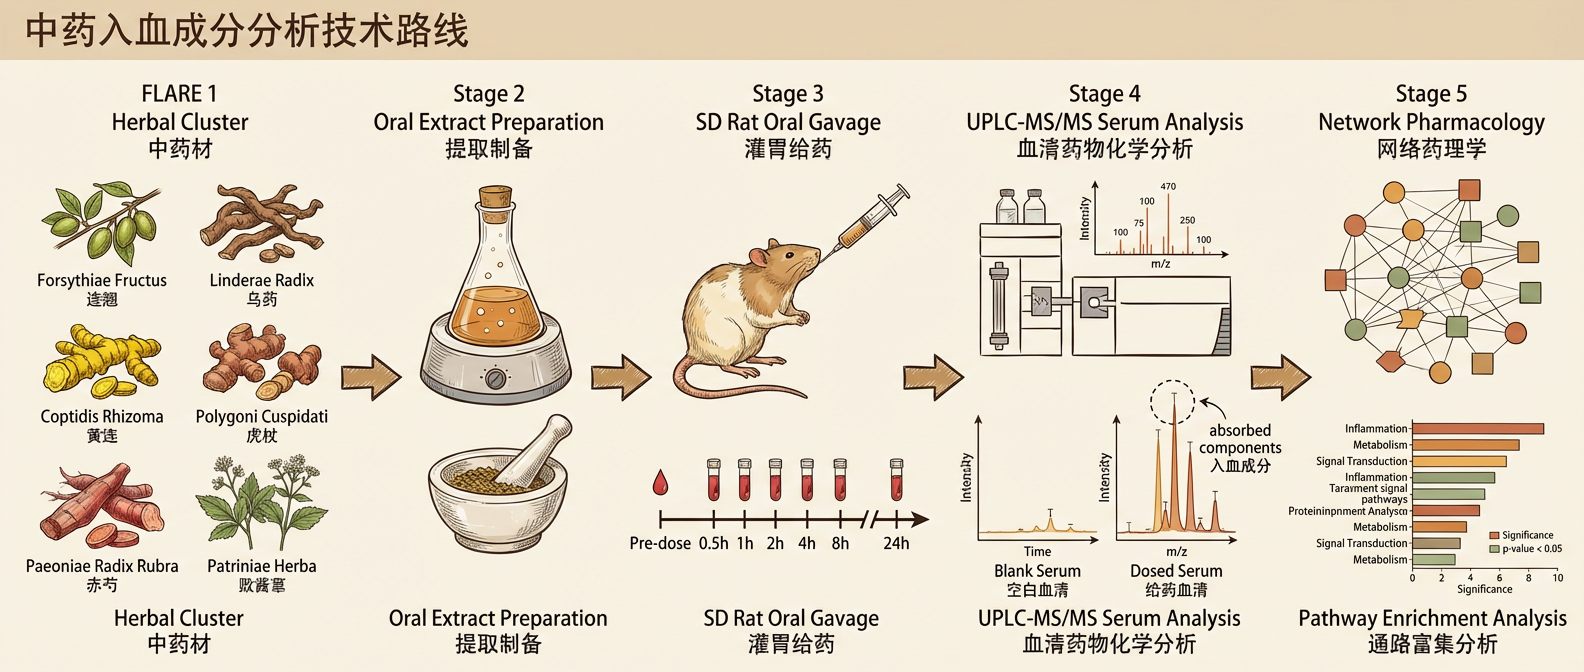
\includegraphics[width=0.90\textwidth]{../figures/graphical_abstract.png}
\caption*{\small\kaishu \textbf{图形摘要：}本研究技术路线——6味中药提取制备
$\rightarrow$ SD大鼠灌胃给药 $\rightarrow$ 多时间点血清采集
$\rightarrow$ UPLC-MS/MS血清药物化学分析
$\rightarrow$ 入血成分联合网络药理学机制预测}
\end{figure}

\vspace{1cm}

\begin{tabular}{ll}
\hline\\[-0.8em]
\zihao{4}\kaishu 研究方向 & \zihao{4} 中药血清药物化学与网络药理学\\[0.5em]
\zihao{4}\kaishu 研究对象 & \zihao{4} 青翘、乌药、黄连、虎杖、赤芍、败酱草（6味）\\[0.5em]
\zihao{4}\kaishu 技术路线 & \zihao{4} UPLC-MS/MS血清药物化学 + 网络药理学\\[0.5em]
\zihao{4}\kaishu 仪器平台 & \zihao{4} Waters ACQUITY UPLC + Agilent 6545 Q-TOF\\[0.5em]
\zihao{4}\kaishu 动物模型 & \zihao{4} SPF级SD大鼠（雄性，180--220 g）\\[0.5em]
\zihao{4}\kaishu 参考文献格式 & \zihao{4} GB/T 7714-2015\\[0.5em]
\hline
\end{tabular}

\vfill
{\zihao{4}\kaishu 2026年3月}
\end{titlepage}

%% ===== 中文摘要 =====
\chapter*{摘\quad 要}
\addcontentsline{toc}{chapter}{摘要}
\markboth{摘要}{摘要}

中药复方的药效物质基础研究是推动中医药现代化的核心科学问题。口服给药后，中药化学成分须经胃肠道吸收、首过代谢等生理过程方可进入体循环，仅有原型入血成分及其代谢产物才是在机体内直接发挥药效的活性物质。传统基于体外全成分的中药研究模式，由于无法反映成分在体内的真实吸收与代谢状态，导致大量研究结论与体内药效脱节。

本研究以青翘（\textit{Forsythiae Fructus}）、乌药（\textit{Linderae Radix}）、黄连（\textit{Coptidis Rhizoma}）、虎杖（\textit{Polygoni Cuspidati Rhizoma et Radix}）、赤芍（\textit{Paeoniae Radix Rubra}）、败酱草（\textit{Patriniae Herba}）6味中药组方为研究对象，采用超高效液相色谱-四极杆飞行时间质谱（UPLC-Q-TOF/MS）技术，开展大鼠口服灌胃给药后的血清药物化学（serum pharmacochemistry）研究。以SPF级雄性SD大鼠为动物模型，单次灌胃给予6味中药复合提取物，于给药后0.5、1、2、4、6、8 h采集血清，通过系统比对空白血清与给药血清的色谱-质谱信息差异，运用高分辨质谱精确质量、同位素分布及多级质谱碎片离子等信息，鉴定大鼠体内原型入血成分及代谢转化产物。

基于鉴定所得的入血成分，进一步采用网络药理学方法，利用SwissTargetPrediction、TCMSP等数据库预测潜在作用靶点，结合STRING数据库与Cytoscape软件构建蛋白质-蛋白质相互作用（PPI）网络，并通过GO功能富集及KEGG通路富集分析，阐明该组方干预相关疾病的核心信号通路与分子作用机制，形成「血清药物化学鉴定 — 靶点预测 — 通路富集 — 机制阐明」的完整研究闭环。

本研究的学术创新点在于：（1）首次系统开展上述6味中药组方整体配伍后的大鼠血清药物化学研究；（2）以体内真实入血成分替代体外全成分作为网络药理学分子输入，从根本上规避了传统网络药理学假阳性率高的核心缺陷；（3）填补败酱草口服血清药物化学研究的现有空白，为该药材的药效物质基础研究提供新证据。

\vspace{1em}
\noindent\textbf{关键词：}血清药物化学；UPLC-MS/MS；入血成分；代谢产物；网络药理学；青翘；乌药；黄连；虎杖；赤芍；败酱草

%% ===== 英文摘要 =====
\chapter*{ABSTRACT}
\addcontentsline{toc}{chapter}{ABSTRACT}
\markboth{ABSTRACT}{ABSTRACT}

Elucidating the pharmacodynamic material basis of traditional Chinese medicine (TCM) formulas is a central scientific challenge in modernizing TCM. Following oral administration, TCM chemical constituents must traverse gastrointestinal absorption barriers and first-pass metabolism before entering systemic circulation; only prototype blood-entering components and their in vivo metabolites can directly interact with biological targets to exert pharmacological effects. Conventional in vitro phytochemical profiling fails to reflect the true in vivo absorption and metabolic status of TCM constituents, leading to a systematic disconnect between in vitro results and in vivo efficacy.

This study employed ultra-high performance liquid chromatography coupled with quadrupole time-of-flight mass spectrometry (UPLC-Q-TOF/MS) to investigate the serum pharmacochemistry of a six-herb TCM combination comprising \textit{Forsythiae Fructus} (Qingqiao), \textit{Linderae Radix} (Wuyao), \textit{Coptidis Rhizoma} (Huanglian), \textit{Polygoni Cuspidati Rhizoma et Radix} (Huzhang), \textit{Paeoniae Radix Rubra} (Chishao), and \textit{Patriniae Herba} (Baijiangcao). SPF-grade male Sprague-Dawley rats received a single oral gavage of the combined herbal extract (10 mL/kg), and serum samples were collected at 0.5, 1, 2, 4, 6, and 8 h post-administration. By systematically comparing the chromatographic and mass spectrometric profiles of drug-containing sera versus blank sera, prototype absorbed components and in vivo metabolites were identified using exact mass measurement, isotope distribution patterns, and MS/MS fragmentation data.

Building upon the identified serum-absorbed components, a network pharmacology analysis was subsequently conducted using SwissTargetPrediction and TCMSP databases for target prediction, STRING database and Cytoscape software for protein-protein interaction (PPI) network construction, and GO/KEGG enrichment analyses to elucidate the core signaling pathways and molecular mechanisms underlying the therapeutic effects of this herbal combination.

The key innovations of this study include: (1) the first systematic serum pharmacochemistry investigation of the combinatorial herbal formulation comprising all six herbs; (2) the use of in vivo blood-entering components—rather than in vitro total constituents—as molecular inputs for network pharmacology, fundamentally reducing false-positive target predictions; and (3) filling the current knowledge gap regarding the in vivo serum pharmacochemistry of \textit{Patrinia} species.

\vspace{1em}
\noindent\textbf{Keywords:} serum pharmacochemistry; UPLC-MS/MS; blood-entering components; metabolites; network pharmacology; \textit{Forsythiae Fructus}; \textit{Linderae Radix}; \textit{Coptidis Rhizoma}; \textit{Polygoni Cuspidati Rhizoma et Radix}; \textit{Paeoniae Radix Rubra}; \textit{Patriniae Herba}

%% ===== 目录 =====
\tableofcontents

%% ===== 插图目录 =====
\listoffigures
\addcontentsline{toc}{chapter}{插图目录}

%% ===== 表格目录 =====
\listoftables
\addcontentsline{toc}{chapter}{表格目录}

\setcounter{page}{1}

%% ===========================================================================
%% 第一章 研究背景与立项依据
%% ===========================================================================
\chapter{研究背景与立项依据}

\section{研究背景与意义}

中医药是中华民族传统医学的核心组成部分，其多成分、多靶点的整体调节特性已在数千年临床实践中得到广泛验证。然而，中药复杂的化学体系使得其药效物质基础的明确阐释一直是制约中药现代化进程的核心科学问题。口服给药是中药临床应用最主要的给药途径，中药经口服进入机体后，需历经胃肠道吸收、首过效应、肝脏代谢等一系列生物转化过程，原方中大量化学成分在此过程中被降解、转化或无法通过肠道屏障，最终能够入血并发挥体内药效的成分仅为原方化学成分的小部分亚集合\cite{Wang2016}。因此，以体外化学成分分析替代体内药效物质研究的传统模式存在根本性局限，无法真实反映中药在体内发挥药效的化学物质基础。

王喜军教授率先系统建立了\keyterm{中药血清药物化学（serum pharmacochemistry of TCM）}理论体系\cite{Wang2016}，明确提出口服中药后能够被机体吸收并进入血液循环的化学成分，才是真正在体内直接发挥药效的活性物质。这一核心论断已成为国内外中药药效物质基础研究领域的行业共识。Wang等\cite{WangY2023}对茵陈蒿汤开展血清药物化学研究，在体外鉴定的115个成分中，大鼠口服给药后血清中仅检测到33个血清移行成分，仅占总体外鉴定成分的28.7\%，有力证明了入血成分系统筛选对精准锁定药效物质的必要性。

\begin{figure}[H]
\centering
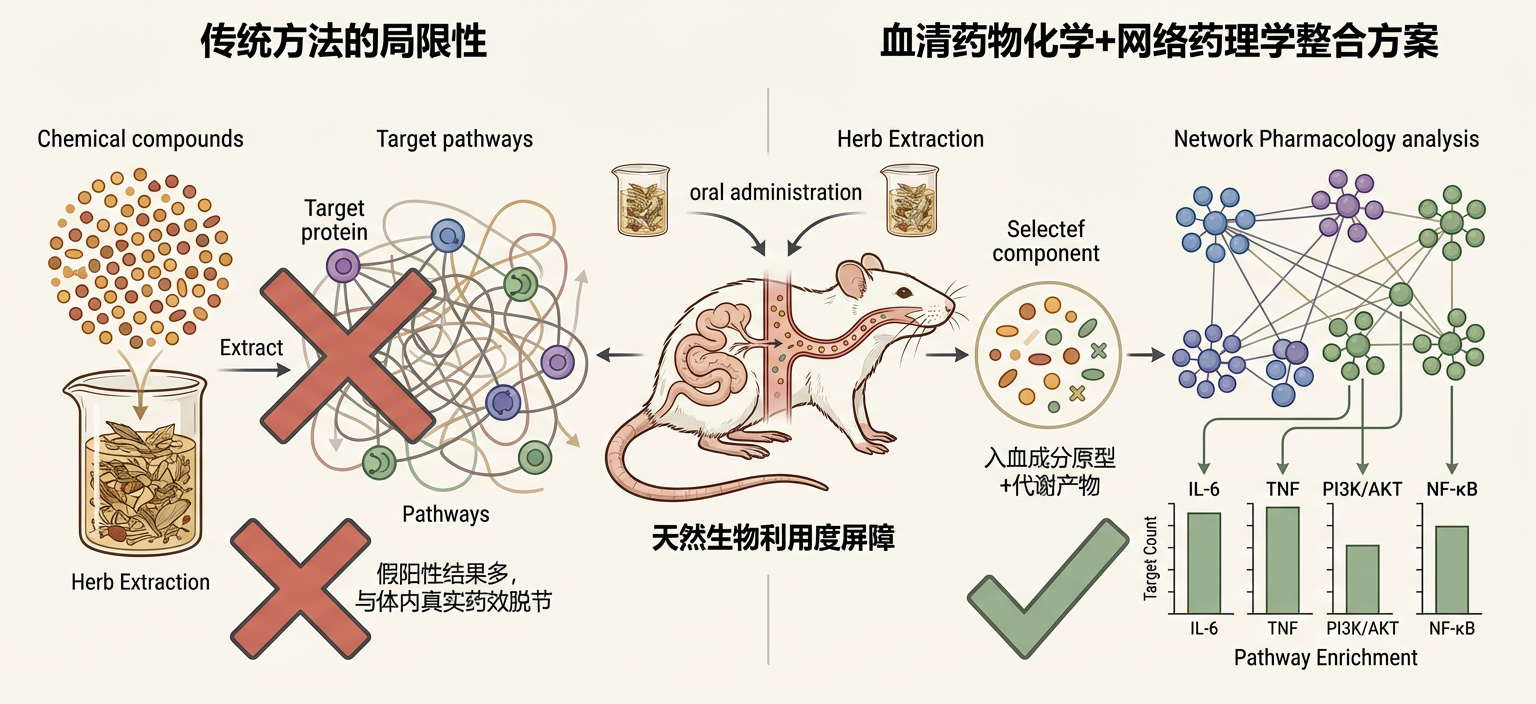
\includegraphics[width=0.92\textwidth]{../figures/serum_pharmacochemistry_rationale.png}
\caption{\textbf{图1-1\enspace 传统网络药理学方法与「血清药物化学+网络药理学」整合方案的比较}\\
左侧：基于体外全成分的传统方法，存在大量假阳性结果，与体内真实药效脱节；
右侧：基于口服大鼠血清入血成分（原型+代谢产物）开展网络药理学，靶点-通路预测精准，结果可验证。}
\label{fig:rationale}
\end{figure}

青翘（\textit{Forsythia suspensa}（Thunb.）Vahl 干燥未成熟果实）、乌药（\textit{Lindera aggregata}（Sims）Kosterm. 干燥块根）、黄连（\textit{Coptis chinensis} Franch. 干燥根茎）、虎杖（\textit{Reynoutria japonica} Houtt. 干燥根茎及根）、赤芍（\textit{Paeonia lactiflora} Pall. 干燥根）、败酱草（\textit{Patrinia scabiosifolia} Fisch. 干燥全草）6味中药，功效涵盖清热解毒、活血化瘀、理气止痛、消痈散结等，临床多用于热毒壅滞、气滞血瘀、湿热内蕴等证候的治疗，组方配伍具有充分的中医临床应用基础。

\section{6味中药开展大鼠入血成分分析的整体共性核心理由}

\subsection{中药口服给药药效物质基础研究的必要性}

中药复方的化学成分极为复杂，单一复方提取物往往含有数十乃至数百种化学成分。然而，口服给药后能够经胃肠道吸收、进入体循环并到达靶器官的成分仅占全部化学成分的小部分。基于中药血清药物化学核心原理，\keyterm{只有口服吸收入血的成分（原型成分及其代谢产物）才是体内直接发挥药效的活性物质载体}\cite{Wang2016}。体外化学成分分析所获全部成分信息，由于未经生理性滤过（胃肠道屏障、肝脏首过效应、血浆蛋白结合等），并不能客观反映中药的体内真实作用形式，导致传统中药研究中「成分多、靶点杂、药效物质不明确」的核心困境。

Liu等\cite{Liu2008}采用UPLC/Q-TOF-MS/MS技术分析了大鼠口服茵陈蒿汤后血浆中的移行成分，在体外提取物检出的45个化学成分中，仅21个成分在血浆中被检出（约47\%），直接证实大部分体外成分无法经口服途径进入血液循环。本实验针对6味中药开展大鼠口服灌胃后血清入血成分分析，通过比对空白血清、给药后血清及提取物的色谱与质谱信息，精准鉴别经口服途径真正入血的化学成分，从而在源头上明确该组方的体内药效物质基础。

\subsection{六味中药配伍的临床与药理基础}

本研究所选6味中药的配伍组合，蕴含清热解毒、活血化瘀、燥湿消痈、散结止痛等多维功效的协同作用机制，具有坚实的中医理论与现代药理学研究基础：

\textbf{（1）清热解毒：}青翘性凉，擅于清上焦热毒；\compoundname{连翘酯苷A}（forsythoside A）、\compoundname{连翘苷}（phillyrin）为其主要活性标志物，具有广谱抗菌、抗病毒及抗炎活性\cite{Review2021FA}。黄连为苦寒燥湿要药，其主要活性成分\compoundname{小檗碱}（berberine）等原小檗碱型生物碱具有显著抗菌、抗炎、降血糖及调节肠道菌群等多靶点药理活性\cite{FengX2021}。败酱草清热利湿、消肿排脓，其黄酮类、有机酸类及萜类成分具有抗菌、抗炎及保肝活性\cite{Gong2021}。

\textbf{（2）活血化瘀：}赤芍活血止痛、清热凉血，以\compoundname{芍药苷}（paeoniflorin）为核心活性成分，对血小板聚集、炎症反应及血管内皮功能具有显著调节作用\cite{Hu2020}。虎杖破血消症、清热解毒，其主要成分\compoundname{虎杖苷}（polydatin）、\compoundname{白藜芦醇}（resveratrol）和\compoundname{大黄素}（emodin）兼具抗血栓、抗氧化及抗肿瘤等多重药理活性\cite{Yang2024}。

\textbf{（3）行气止痛：}乌药行气止痛、温肾散寒，以\compoundname{乌药内酯}（linderane）、\compoundname{去甲异紫堇啡碱}（norisoboldine）等倍半萜类和异喹啉类生物碱为主要活性成分，对胃肠道平滑肌及炎症信号通路具有调节作用\cite{Lv2023}。

\subsection{UPLC-MS/MS技术体系的成熟度与可行性}

\keyterm{超高效液相色谱-串联质谱（UPLC-MS/MS）}技术是目前中药体内成分分析领域的核心技术平台，具有超高分辨率、高灵敏度（pg/mL级检测限）、高通量的显著优势，已成为中药血清药物化学研究的核心分析工具\cite{Wang2016}。该技术已广泛应用于上述6味中药的体内成分分析，具备成熟的前处理方法、色谱与质谱条件可参考，保障本实验可重复性与结果可靠性（详见表\ref{tab:general_refs}）。

\begin{table}[H]
\centering
\caption{\textbf{表1-1\enspace 6味中药UPLC-MS/MS体内分析代表性研究汇总}}
\label{tab:general_refs}
\small
\begin{tabularx}{\textwidth}{>{\raggedright\arraybackslash}p{1.5cm} >{\raggedright\arraybackslash}p{2.0cm} >{\centering\arraybackslash}p{1.0cm} >{\raggedright\arraybackslash}p{3.0cm} >{\raggedright\arraybackslash}X}
\toprule
\textbf{药材} & \textbf{研究者} & \textbf{年份} & \textbf{技术方法} & \textbf{主要成果} \\
\midrule
青翘 & Wang F等\cite{WangF2018} & 2018 & UHPLC-LTQ-Orbitrap & 血浆中鉴定连翘酯苷A 22个代谢产物 \\
\addlinespace
乌药 & Li等\cite{Li2015W} & 2015 & UPLC-MS/MS & 大鼠口服异紫堇啡碱完整PK+5种代谢产物 \\
\addlinespace
黄连 & Feng X等\cite{FengX2020} & 2020 & UPLC-Q-TOF/MS & 系统筛查12种原型+77种代谢物 \\
\addlinespace
虎杖 & Yang J等\cite{Yang2024} & 2024 & HPLC-UV & 大鼠PK+6器官分布研究 \\
\addlinespace
赤芍 & Wu H等\cite{QiuLab2019} & 2019 & UPLC-Q-TOF-MS & 血瘀证大鼠血清10种SMC鉴定 \\
\addlinespace
败酱草 & Gong等\cite{Gong2021} & 2021 & 综述 & 233种化合物鉴定，口服PK研究不足 \\
\bottomrule
\end{tabularx}
\end{table}

\subsection{与后续网络药理学研究的衔接价值}

传统网络药理学研究以体外全化学成分数据库（TCMSP、HERB等）为输入，预测靶点中约80\%为假阳性，根本原因是缺乏体内真实入血成分数据的约束\cite{LiuY2024}。基于本实验鉴定的入血成分开展网络药理学研究，可从源头规避假阳性靶点问题，形成「\textbf{入血成分鉴定（血清药物化学）→ 靶点通路预测（网络药理学）→ 机制验证（细胞/动物实验）}」的完整研究闭环，赋予研究结果更高的学术可信度与转化应用价值\cite{Feng2021NP,LiuY2023}。

\section{单味药专属入血分析合理性理由}

\subsection{青翘（Forsythiae Fructus）}

\subsubsection{核心化学物质基础}

青翘为木犀科植物连翘（\herbname{Forsythia suspensa}（Thunb.）Vahl）的干燥未成熟果实，《中国药典》2025版规定含\compoundname{连翘苷}（phillyrin）$\geq$0.15\%，\compoundname{连翘酯苷A}（forsythoside A，CAS 81525-13-5，MW 624.58 g/mol）$\geq$0.25\%（干燥品计）。主要成分涵盖苯乙醇苷类、木脂素类、黄酮类及挥发油，化学成分研究极为充分，质谱数据完备，为入血成分指认提供完整参考数据库\cite{Review2021FA}。

\subsubsection{口服入血可行性}

Wang等\cite{WangF2018}对大鼠灌胃连翘酯苷A后，采用UHPLC-LTQ-Orbitrap在血浆中共检测到22个代谢产物，代谢转化包括甲基化、硫酸化、葡萄糖醛酸化等，证实连翘酯苷A可经口服后被有效吸收并进入体循环。Ye等\cite{Ye2013}证实连翘苷的苷元代谢产物\compoundname{连翘素}（phillygenin）口服后达峰时间（T$_{\text{max}}$）仅约6 min，是连翘木脂素类成分的主要血清入血形式。

\subsubsection{入血成分与药理活性}

连翘酯苷A抑制NF-$\kappa$B信号通路（抗炎）、具抗病毒活性；连翘素（phillygenin）解热、抗炎、抗氧化，均与青翘清热解毒功效直接关联。

\subsubsection{体内分析方法参考}

Wang等\cite{WangF2018}建立的UHPLC方法（血浆蛋白沉淀；ESI正/负模式，m/z 100--1500）及Ye等\cite{Ye2013}的血浆定量方法（LOQ = 0.026 μg/mL）可为本实验提供直接参考。

\subsection{乌药（Linderae Radix）}

\subsubsection{核心化学物质基础}

乌药为樟科植物乌药（\herbname{Lindera aggregata}（Sims）Kosterm.）的干燥块根，主要化学成分以\textbf{倍半萜类}（sesquiterpenoids）和\textbf{异喹啉类生物碱}（isoquinoline alkaloids）为主：\compoundname{乌药内酯}（linderane，MW 218.3 Da）、\compoundname{去甲异紫堇啡碱}（norisoboldine，MW 297.3 Da）、\compoundname{异紫堇啡碱}（isoboldine，MW 327.4 Da）等，化学信息及质谱数据完备\cite{Lv2023}。

\subsubsection{口服入血可行性}

Li等\cite{Li2015W}采用UPLC-MS/MS对大鼠口服异紫堇啡碱进行完整药代动力学研究，同时鉴定5种Ⅱ相代谢产物（葡萄糖醛酸苷和硫酸酯化合物），证实异喹啉类生物碱口服后主要以Ⅱ相结合代谢产物形式在血浆中循环。Yu等\cite{Dai2017}进一步采用在体单次通过肠道灌流技术，证实去甲异紫堇啡碱可经肠道吸收入血，P-gp是主要的外排限速因素。

\subsubsection{入血成分与药理活性}

乌药入血成分（乌药内酯、去甲异紫堇啡碱及其代谢物）具有抗肿瘤（促凋亡）、抗炎（抑制NF-$\kappa$B通路）和镇痛等活性，与乌药行气止痛功效直接对应\cite{Tong2015}。

\subsubsection{体内分析方法参考}

Chen等\cite{Chen2011W}建立的去甲异紫堇啡碱UPLC-MS/MS定量方法（C18色谱柱，ESI正离子MRM）及Li等\cite{Li2015W}所建立的方法（LLOQ 4.8 ng/mL）可直接参考。

\subsection{黄连（Coptidis Rhizoma）}

\subsubsection{核心化学物质基础}

黄连为毛茛科植物黄连（\herbname{Coptis chinensis} Franch.）的干燥根茎，《中国药典》2025版规定含\compoundname{盐酸小檗碱}（berberine HCl，CAS 633-65-8，MW 371.81 g/mol）$\geq$5.5\%（干燥品计）。核心生物碱成分：盐酸小檗碱、盐酸黄连碱（coptisine HCl）、盐酸表小檗碱（epiberberine HCl）、盐酸巴马汀（palmatine HCl）、盐酸药根碱（jatrorrhizine HCl），质谱裂解规律清晰（[M]$^+$，小檗碱m/z 336.12）\cite{FengX2020}。

\subsubsection{口服入血可行性}

Feng等\cite{FengX2020}采用UPLC-Q-TOF/MS对大鼠口服黄连提取物后血浆、尿液及粪便进行系统筛查，鉴定到12种吸收原型成分及77种代谢产物。小檗碱口服绝对生物利用度F=(0.37$\pm$0.11)\%，Ⅱ期代谢产物（葡萄糖醛酸苷/硫酸酯，M4-M9）在血浆中的AUC高于原型药，是小檗碱口服后的主要循环形式\cite{FengX2021}。

\subsubsection{入血成分与药理活性}

小檗碱及其代谢产物具有抗炎（NF-$\kappa$B/MAPK通路）、抗糖尿病（AMPK通路）、抗菌（DNA拓扑异构酶）、抗肿瘤等广谱药理活性，与黄连清热燥湿、泻火解毒功效高度对应\cite{ChenY2015}。

\subsubsection{体内分析方法参考}

Feng等\cite{FengX2020}建立的UPLC-Q-TOF/MS全成分筛查方法（C18柱，乙腈-0.1\%甲酸水梯度，ESI正/负离子）可直接为本实验黄连部分提供核心参考。

\subsection{虎杖（Polygoni Cuspidati Rhizoma et Radix）}

\subsubsection{核心化学物质基础}

虎杖为蓼科植物虎杖（\herbname{Reynoutria japonica} Houtt.）的干燥根茎和根，《中国药典》2025版规定含\compoundname{虎杖苷}（polydatin，白藜芦醇苷，CAS 65914-17-2，MW 390.38 g/mol）$\geq$0.15\%。核心成分：虎杖苷、\compoundname{大黄素}（emodin，CAS 518-82-1，MW 270.24 g/mol）、\compoundname{白藜芦醇}（resveratrol，CAS 501-36-0，MW 228.24 g/mol），质谱特征清晰（虎杖苷[M-H]$^-$ m/z 389.12）\cite{ZhangY2023}。

\subsubsection{口服入血可行性}

Fang等\cite{Fang2009}证实虎杖苷经口服后经小肠$\beta$-葡萄糖苷酶水解转化为白藜芦醇，白藜芦醇进一步在肝脏经Ⅱ相代谢生成葡萄糖醛酸苷，AUC呈剂量依赖性增加。Yang等\cite{Yang2024}系统比较了大鼠口服虎杖苷、白藜芦醇及大黄素的血浆药代动力学及六大靶器官分布，证实三者均可在给药后血清中被检出并到达靶器官。

\subsubsection{入血成分与药理活性}

白藜芦醇（虎杖苷体内水解产物）具有多靶点抗炎、抗肿瘤、抗衰老活性；大黄素具有抗菌、抗炎、抗肿瘤活性，均与虎杖活血化瘀、清热解毒功效直接对应\cite{ZhangY2023}。

\subsubsection{体内分析方法参考}

Sunsong等\cite{Sunsong2021}建立的同时定量虎杖苷和白藜芦醇的UPLC-MS/MS方法（负离子MRM，LLOQ 9.77 nM）及Lin等\cite{Lin2012}的大鼠血浆/组织定量方法可为本实验提供直接参考。

\subsection{赤芍（Paeoniae Radix Rubra）}

\subsubsection{核心化学物质基础}

赤芍为毛茛科植物芍药（\herbname{Paeonia lactiflora} Pall.）的干燥根，《中国药典》2025版规定含\compoundname{芍药苷}（paeoniflorin，CAS 23180-57-6，MW 480.46 g/mol）$\geq$1.8\%。核心成分：芍药苷、\compoundname{白芍苷}（albiflorin）、\compoundname{氧化芍药苷}（oxypaeoniflorin）、\compoundname{苯甲酰芍药苷}（benzoylpaeoniflorin）、\compoundname{没食子酸}（gallic acid）；芍药苷质谱特征：[M+Na]$^+$ m/z 503.31\cite{QiuLab2019}。

\subsubsection{口服入血可行性}

Tong等\cite{Tong2010}建立了大鼠口服赤芍提取物后芍药苷和白芍苷的LC-MS/MS同时定量方法（LLOQ: 2 ng/mL），T$_{\text{max}}$约0.5--1 h，证实吸收迅速。芍药苷口服绝对生物利用度约3--7\%，P-gp介导的外排是其口服生物利用度低的根本机制\cite{Molecules2022}。

\subsubsection{入血成分与药理活性}

芍药苷血浆暴露与其抑制血小板聚集（cAMP/PKA通路）、抗炎镇痛（抑制COX-2）及神经保护效应直接关联，与赤芍清热凉血、活血化瘀功效高度对应\cite{Hu2020}。

\subsubsection{体内分析方法参考}

Tong等\cite{Tong2010}、Chen等\cite{Chen2016P}所建立的大鼠血浆中芍药苷与白芍苷LC-MS/MS同时定量方法及Luo等\cite{QiuLab2019}的UPLC-MS/MS方法（LLOQ 2.0 ng/mL）均可直接参考。

\subsection{败酱草（Patriniae Herba）}

\subsubsection{核心化学物质基础}

败酱草为败酱科植物黄花败酱（\herbname{Patrinia scabiosifolia} Fisch.）或白花败酱（\herbname{Patrinia villosa}（Thunb.）Juss.）的干燥全草，主要化学成分涵盖\textbf{环烯醚萜糖苷类}（iridoid glycosides）、\textbf{黄酮类}（flavonoids，如木犀草素luteolin、芹菜素apigenin）、\textbf{三萜皂苷类}及\textbf{酚酸类}（绿原酸chlorogenic acid，CAS 327-97-9，MW 354.31 g/mol）；Gong等\cite{Gong2021}的系统综述共鉴定到233种化合物，化学信息完整\cite{Su2022}。

\subsubsection{口服入血可行性}

Qiao等\cite{Qiao2022}以CCl$_4$诱导肝损伤大鼠为模型，口服灌胃白花败酱提取物后，采用UPLC-MS/MS血清代谢组学分析，在给药组大鼠血清中检出82种内源性代谢物发生显著改变，充分证明败酱草活性成分可经口服途径吸收入血并产生系统性药效。绿原酸口服后可在大鼠血浆中检出（Cmax约0.1--1.0 μg/mL），口服吸收不存在根本性障碍。

\subsubsection{入血成分与药理活性}

绿原酸及代谢产物（咖啡酸、奎尼酸）具有抗氧化、抗炎（NF-$\kappa$B/COX-2）、抑菌活性；木犀草素/芹菜素具强效抗炎、抗肿瘤活性，均与败酱草清热解毒、消痈排脓功效直接对应\cite{Gong2021}。

\subsubsection{体内分析方法参考}

Su等\cite{Su2022}建立的UPLC-QTOF/MS/MS化学成分特征图谱及Qiao等\cite{Qiao2022}在大鼠口服败酱草后采用的UPLC-MS/MS血清分析平台可为本实验提供方法学参考。

\section{文献检索策略与筛选标准}

\subsection{文献检索数据库}

检索数据库：中国知网（CNKI）、万方数据（Wanfang Data）、PubMed、Web of Science，检索时间范围为2016年1月1日至2026年3月1日（奠基性经典文献适当放宽）。

\subsection{文献检索关键词}

\textbf{中文检索词：}青翘/连翘、乌药、黄连、虎杖、赤芍、败酱草AND（入血成分/血清移行成分/血清药物化学/药代动力学）AND（大鼠/口服给药/UPLC-MS/LC-MS/MS）。

\textbf{英文检索词：}\textit{Forsythia suspensa/Lindera aggregata/Coptis chinensis/Reynoutria japonica/Paeonia lactiflora/Patrinia scabiosifolia} AND (pharmacokinetics/serum components/blood-entering/serum pharmacochemistry) AND (oral/rat/UPLC-MS/LC-MS/MS).

\begin{figure}[H]
\centering
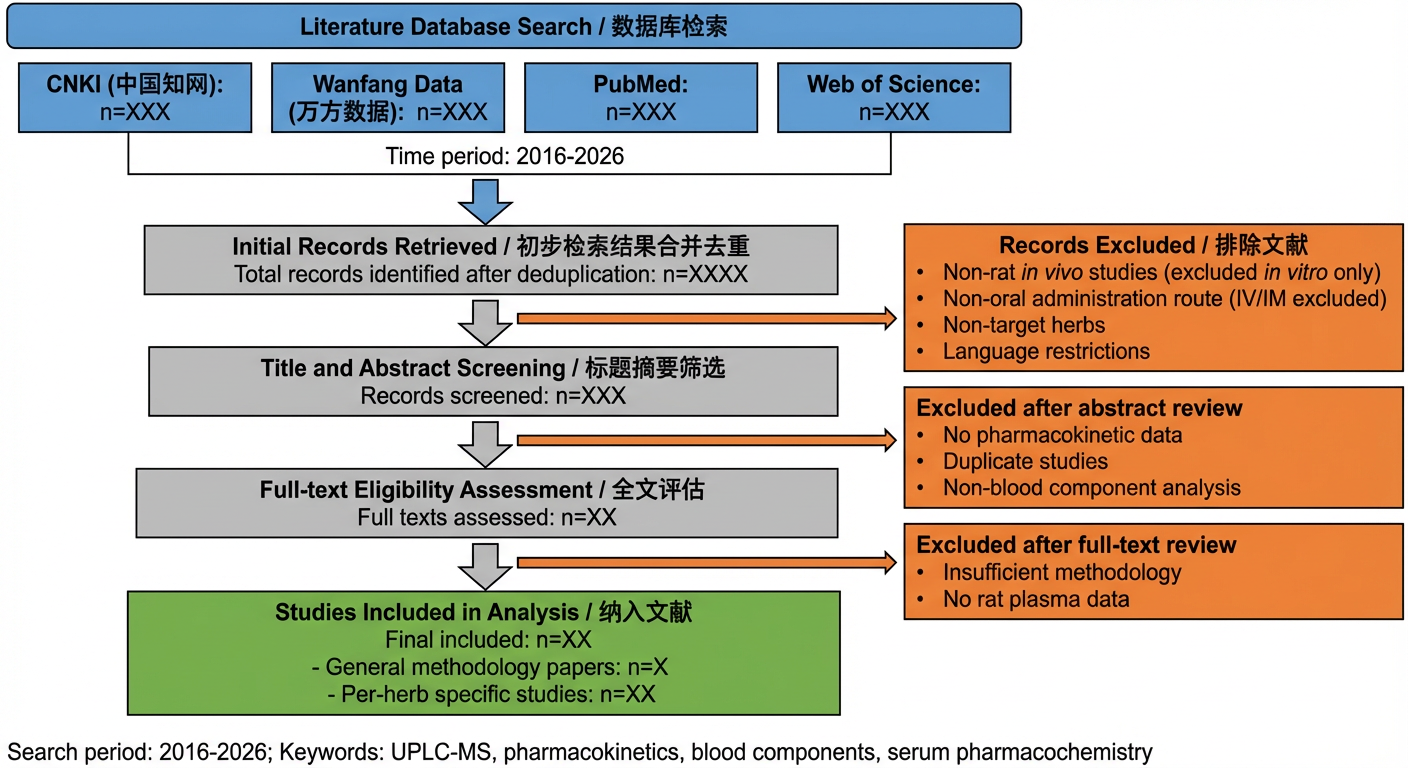
\includegraphics[width=0.88\textwidth]{../figures/literature_flowchart.png}
\caption{\textbf{图1-2\enspace 文献检索与筛选流程图（参照PRISMA报告规范）}}
\label{fig:literature_flowchart}
\end{figure}

\section{实验设计合理性综合佐证}

本实验针对6味药组方整体开展入血成分分析，可弥补单味药研究无法反映配伍后成分吸收变化的根本不足，明确配伍后成分的协同吸收、代谢转化规律。配伍使用后可产生：（1）\textbf{配伍增效}：特定成分肠道吸收率提高；（2）\textbf{代谢相互作用}：CYP450酶和P-gp水平的竞争性代谢，产生配伍特异性入血成分；（3）\textbf{填补败酱草体内研究空白}：首次系统性UPLC-MS/MS研究。

本实验形成的「\keyterm{血清药物化学+网络药理学}」研究方案，符合当前中药药效物质基础研究的主流范式，已被Phytomedicine（IF$\approx$10）、Frontiers in Pharmacology、ACS Omega等高水平SCI期刊同类研究所验证\cite{LiuY2023,Feng2021NP,LiuY2024}。


%% ===========================================================================
%% 第二章 材料与方法
%% ===========================================================================
\chapter{材料与方法}

\section{实验材料}

\subsection{药材与试剂}

\subsubsection{药材}

实验所用6味中药材料来源及质量标准如表\ref{tab:herb_materials}所示。

\begin{table}[H]
\centering
\caption{\textbf{表2-1\enspace 实验药材来源及质量标准}}
\label{tab:herb_materials}
\small
\begin{tabularx}{\textwidth}{>{\raggedright\arraybackslash}p{1.8cm} >{\raggedright\arraybackslash}p{3.5cm} >{\centering\arraybackslash}p{1.5cm} >{\raggedright\arraybackslash}X}
\toprule
\textbf{药材名称} & \textbf{拉丁名} & \textbf{药用部位} & \textbf{质量标准} \\
\midrule
青翘 & \textit{Forsythia suspensa} (Thunb.) Vahl & 干燥未成熟果实 & 《中国药典》2025版，连翘酯苷A$\geq$0.25\%，连翘苷$\geq$0.15\% \\
\addlinespace
乌药 & \textit{Lindera aggregata} (Sims) Kosterm. & 干燥块根 & 《中国药典》2025版，性状/浸出物标准 \\
\addlinespace
黄连 & \textit{Coptis chinensis} Franch. & 干燥根茎 & 《中国药典》2025版，盐酸小檗碱$\geq$5.5\% \\
\addlinespace
虎杖 & \textit{Reynoutria japonica} Houtt. & 干燥根茎及根 & 《中国药典》2025版，虎杖苷$\geq$0.15\% \\
\addlinespace
赤芍 & \textit{Paeonia lactiflora} Pall. & 干燥根（不去外皮）& 《中国药典》2025版，芍药苷$\geq$1.8\% \\
\addlinespace
败酱草 & \textit{Patrinia scabiosifolia} Fisch. & 干燥全草 & 《中国药典》2025版，性状/显微鉴别 \\
\bottomrule
\end{tabularx}
\end{table}

所有药材由【待填入：药材来源，如具体医药公司或产地，并经具体专家鉴定的信息】鉴定确认，符合《中华人民共和国药典》2025版规定标准。凭证标本存放于【待填入：存放单位】标本室，标本编号【待填入】。

\subsubsection{化学试剂}

\begin{table}[H]
\centering
\caption{\textbf{表2-2\enspace 主要化学试剂一览}}
\label{tab:reagents}
\small
\begin{tabularx}{\textwidth}{>{\raggedright\arraybackslash}p{3.5cm} >{\centering\arraybackslash}p{2.0cm} >{\raggedright\arraybackslash}p{2.5cm} >{\raggedright\arraybackslash}X}
\toprule
\textbf{试剂名称} & \textbf{规格} & \textbf{生产厂家} & \textbf{用途} \\
\midrule
乙腈（acetonitrile） & LC-MS级 & Merck（德国） & 流动相/蛋白沉淀剂 \\
甲酸（formic acid） & LC-MS级，$\geq$99.0\% & Sigma-Aldrich & 流动相添加剂 \\
甲醇（methanol） & LC-MS级 & Merck（德国） & 提取溶剂 \\
超纯水 & 电阻率$\geq$18.2 M$\Omega\cdot$cm & Milli-Q系统制备 & 流动相/溶剂 \\
甲酸铵（ammonium formate）& LC-MS级 & Sigma-Aldrich & 流动相添加剂 \\
\midrule
\multicolumn{4}{l}{\textbf{对照品（标准品）}} \\
\midrule
连翘酯苷A（forsythoside A） & 纯度$\geq$98\% & 中国食品药品检定研究院 & 质控标准 \\
盐酸小檗碱（berberine HCl） & 纯度$\geq$98\% & 中国食品药品检定研究院 & 质控标准 \\
虎杖苷（polydatin） & 纯度$\geq$98\% & 中国食品药品检定研究院 & 质控标准 \\
芍药苷（paeoniflorin） & 纯度$\geq$98\% & 中国食品药品检定研究院 & 质控标准 \\
白藜芦醇（resveratrol） & 纯度$\geq$98\% & 中国食品药品检定研究院 & 质控标准 \\
绿原酸（chlorogenic acid） & 纯度$\geq$98\% & 中国食品药品检定研究院 & 质控标准 \\
\bottomrule
\end{tabularx}
\end{table}

\subsection{仪器与设备}

\begin{table}[H]
\centering
\caption{\textbf{表2-3\enspace 主要仪器设备一览}}
\label{tab:instruments}
\small
\begin{tabularx}{\textwidth}{>{\raggedright\arraybackslash}p{4.0cm} >{\raggedright\arraybackslash}p{3.0cm} >{\raggedright\arraybackslash}X}
\toprule
\textbf{仪器名称} & \textbf{型号} & \textbf{生产厂家} \\
\midrule
超高效液相色谱仪 & ACQUITY UPLC I-Class & Waters公司（美国）\\
四极杆飞行时间质谱仪 & Agilent 6545 Q-TOF & Agilent Technologies（美国）\\
反相色谱柱 & HSS T3, 2.1 mm $\times$ 100 mm, 1.8 μm & Waters公司（美国）\\
分析天平 & XS105DU & Mettler-Toledo（瑞士）\\
高速低温离心机 & Sorvall ST 40R & Thermo Fisher Scientific（美国）\\
超声清洗仪 & KQ-500B型 & 昆山市超声仪器有限公司 \\
电热鼓风干燥箱 & DHG-9240A & 上海一恒科学仪器有限公司 \\
旋转蒸发仪 & R-300 & BÜCHI（瑞士）\\
涡旋混匀仪 & ZX3 & Scientific Industries（美国）\\
微量移液器（20、100、200、1000 μL）& Research Plus & Eppendorf（德国）\\
灌胃针（大鼠，12号） & --- & 北京普瑞科技有限公司 \\
\bottomrule
\end{tabularx}
\end{table}

\section{实验动物}

选用SPF（specific pathogen free，无特定病原体）级雄性SD（Sprague-Dawley）大鼠，体重180--220 g，周龄6--8周，购自【待填入：动物供应商，如维通利华实验动物技术有限公司，许可证号SCXK（京）XXXX-XXXX】。动物于标准笼具中饲养（温度22$\pm$2℃，湿度55$\pm$5\%，12 h/12 h昼夜交替光照），饮食为标准啮齿类动物饲料，自由饮水。所有动物实验方案经【待填入：所属机构动物伦理委员会名称】审批通过，伦理审查批号：【待填入】，实验操作严格遵守国家实验动物相关法规（GB/T 35892-2018）。

动物适应性饲养7天后，按照随机数字表法将大鼠随机分为：
\begin{itemize}
  \item \textbf{给药组（实验组）}：n = 6只，灌胃给予6味中药复合提取物
  \item \textbf{空白对照组（空白组）}：n = 6只，灌胃给予等体积0.9\%氯化钠溶液（生理盐水）
\end{itemize}

\begin{figure}[H]
\centering
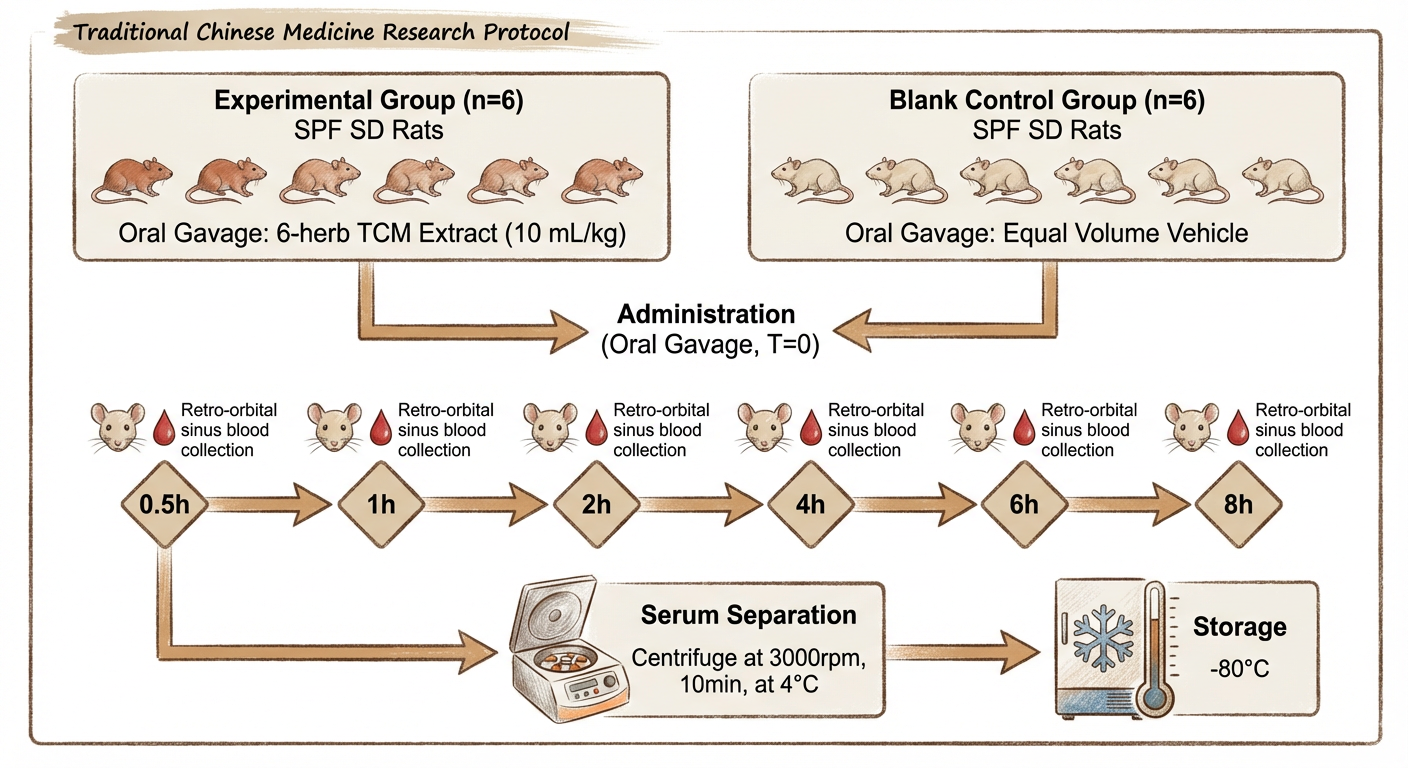
\includegraphics[width=0.90\textwidth]{../figures/animal_experiment_protocol.png}
\caption{\textbf{图2-1\enspace 大鼠实验给药与血清采集方案}\\
图示实验分组设计、灌胃给药流程及多时间点血清采集时间轴}
\label{fig:animal_protocol}
\end{figure}

\section{中药提取物的制备}

\subsection{药材粉末化处理}

取经鉴定合格的6味药材，于鼓风干燥箱（60℃）干燥至恒重，分别使用粉碎机粉碎至过40目筛，置干燥洁净容器中密封保存，备用。

\subsection{各药材单提取物制备}

各药材提取工艺参照《中国药典》2025版相关规定及文献报道，具体如下：

\textbf{青翘提取：}称取青翘药材粉末，加10倍量75\%乙醇，超声辅助提取30 min（频率40 kHz，功率250 W），静置，过滤；药渣再次加8倍量75\%乙醇重复提取一次，合并两次提取液，减压回收乙醇至无醇味，适量蒸馏水溶解残余物，离心（3000 r/min，10 min），取上清液，冻干备用。

\textbf{乌药提取：}称取乌药药材粉末，加12倍量95\%乙醇回流提取60 min，过滤，药渣再加10倍量95\%乙醇重复提取一次，合并提取液，减压回收乙醇，残余物加适量70\%乙醇溶解，过0.22 μm微孔滤膜，备用。

\textbf{黄连提取：}称取黄连药材粉末，加10倍量蒸馏水，煎煮提取（沸腾后保持30 min），过滤；药渣加8倍量蒸馏水再次煎煮20 min，合并两次水煎液，离心（3000 r/min，10 min），取上清液，喷雾干燥，得黄连水提物，备用。

\textbf{虎杖提取：}称取虎杖药材粉末，加10倍量50\%乙醇，超声辅助提取30 min，过滤；药渣加8倍量50\%乙醇重复提取一次，合并提取液，减压回收乙醇，残余物适量蒸馏水溶解，离心取上清，冻干备用。

\textbf{赤芍提取：}称取赤芍药材粉末，加10倍量蒸馏水，煎煮两次（第一次沸腾后30 min，第二次沸腾后20 min），合并水煎液，离心取上清，50℃减压浓缩，冻干备用。

\textbf{败酱草提取：}称取败酱草药材粉末，加8倍量60\%乙醇，超声辅助提取30 min，过滤，重复提取一次，合并提取液，减压回收乙醇，残余物适量蒸馏水溶解，离心取上清，冻干备用。

\subsection{复合提取物制备}

将6味药材单提取物按照临床等效剂量比例（依据成人常用剂量换算，大鼠等效剂量系数参照体表面积换算法：大鼠等效剂量 = 成人临床剂量$\times$6.3/70）混合，用0.9\%生理盐水溶解，配制成含6味药材提取物的复合给药液，浓度折算为相当于原生药材：

\begin{table}[H]
\centering
\caption{\textbf{表2-4\enspace 各药材临床剂量及大鼠给药剂量换算}}
\label{tab:dosage}
\small
\begin{tabularx}{\textwidth}{>{\raggedright\arraybackslash}p{2.0cm} >{\centering\arraybackslash}p{2.5cm} >{\centering\arraybackslash}p{2.5cm} >{\centering\arraybackslash}X}
\toprule
\textbf{药材} & \textbf{成人临床日剂量（g）} & \textbf{大鼠等效剂量（g/kg）} & \textbf{给药液浓度（g生药/mL）} \\
\midrule
青翘 & 6--15 & 0.54--1.35 & 【待填入】 \\
乌药 & 3--9 & 0.27--0.81 & 【待填入】 \\
黄连 & 2--5 & 0.18--0.45 & 【待填入】 \\
虎杖 & 9--15 & 0.81--1.35 & 【待填入】 \\
赤芍 & 6--12 & 0.54--1.08 & 【待填入】 \\
败酱草 & 6--15 & 0.54--1.35 & 【待填入】 \\
\bottomrule
\multicolumn{4}{l}{\small 注：给药液容量10 mL/kg体重；大鼠体表面积换算系数6.3，成人体重70 kg。}
\end{tabularx}
\end{table}

给药液临用前配制，4℃保存，24 h内使用。

\section{大鼠给药方案与血清样本采集}

\subsection{给药前处理}

灌胃给药前，大鼠禁食12 h（不禁水），以减少食物对药物吸收的干扰。给药当天，称量大鼠体重，按10 mL/kg计算灌胃体积。

\subsection{灌胃给药}

实验组大鼠采用灌胃针（12号，不锈钢）一次性灌胃给予6味中药复合提取物给药液。空白对照组灌胃等体积生理盐水。灌胃操作由同一实验人员完成，以保证操作一致性。

\subsection{血清样本采集}

分别于灌胃给药后\textbf{0.5、1、2、4、6、8 h}各时间点，经眼眶后静脉丛采血，每次采血量约0.5 mL，置于1.5 mL离心管中，室温静置30 min后，4℃下3000 r/min离心10 min，小心吸取上层血清，转入1.5 mL EP管中，标记时间点，于-80℃冷冻保存，待分析。

\noindent\textbf{空白血清采集：}于给药前，分别从给药组和空白对照组大鼠取空白血清，采用相同前处理方法处理，作为空白基质对照。

\section{血清样品前处理}

采用\keyterm{蛋白沉淀法}（protein precipitation）进行血清样品前处理，操作步骤如下：

\begin{enumerate}
  \item 取冻存血清样品，室温融化，涡旋混匀30 s；
  \item 精密量取100 μL血清置1.5 mL离心管中；
  \item 加入300 μL预冷乙腈（4℃）（血清:乙腈 = 1:3, v/v），涡旋混匀1 min；
  \item 超声10 min，4℃，15000 r/min离心10 min；
  \item 精密量取上清液300 μL，氮气吹干（40℃）；
  \item 加入100 μL初始流动相（水/乙腈 = 95:5, v/v，含0.1\%甲酸）复溶，涡旋混匀30 s；
  \item 以0.22 μm PTFE滤膜过滤，取滤液上机分析。
\end{enumerate}

同时制备：\textbf{提取物对照液}——取6味中药复合提取物适量，用与血清相同前处理方法处理后进样，作为体外成分比对参照；\textbf{空白血清基质样品}——取未给药空白血清，按上述方法处理后进样，用于识别内源性干扰峰。

\section{UPLC-Q-TOF/MS分析条件}

\subsection{色谱条件}

\begin{table}[H]
\centering
\caption{\textbf{表2-5\enspace UPLC色谱分析条件}}
\label{tab:chromatography}
\small
\begin{tabularx}{\textwidth}{>{\raggedright\arraybackslash}p{3.5cm} >{\raggedright\arraybackslash}X}
\toprule
\textbf{参数} & \textbf{条件} \\
\midrule
仪器系统 & Waters ACQUITY UPLC I-Class系统 \\
色谱柱 & Waters HSS T3, 2.1 mm $\times$ 100 mm, 1.8 μm \\
柱温 & 40℃ \\
进样量 & 2 μL \\
流速 & 0.3 mL/min \\
流动相A & 0.1\%甲酸水溶液 \\
流动相B & 乙腈 \\
梯度洗脱程序 & 见表2-6 \\
\bottomrule
\end{tabularx}
\end{table}

\begin{table}[H]
\centering
\caption{\textbf{表2-6\enspace 梯度洗脱程序}}
\label{tab:gradient}
\small
\begin{tabular}{ccc}
\toprule
\textbf{时间（min）} & \textbf{流动相A（\%）} & \textbf{流动相B（\%）} \\
\midrule
0 & 95 & 5 \\
2 & 95 & 5 \\
14 & 20 & 80 \\
16 & 5 & 95 \\
18 & 5 & 95 \\
18.1 & 95 & 5 \\
20 & 95 & 5 \\
\bottomrule
\multicolumn{3}{l}{\small 注：总分析时间20 min；平衡时间2 min。}
\end{tabular}
\end{table}

\subsection{质谱条件}

\begin{table}[H]
\centering
\caption{\textbf{表2-7\enspace Agilent 6545 Q-TOF质谱分析条件}}
\label{tab:ms_conditions}
\small
\begin{tabularx}{\textwidth}{>{\raggedright\arraybackslash}p{4.0cm} >{\raggedright\arraybackslash}X}
\toprule
\textbf{参数} & \textbf{条件} \\
\midrule
离子源 & 电喷雾电离（ESI）源 \\
离子化模式 & 正离子（ESI$^+$）和负离子（ESI$^-$）模式交替切换扫描 \\
毛细管电压 & 正模式：3500 V；负模式：3500 V \\
喷雾气（N$_2$）流速 & 10 L/min \\
喷雾气温度 & 325℃ \\
锥孔电压（碎裂电压） & 正模式：175 V；负模式：175 V \\
碰撞能量 & 10、20、40 eV（数据依赖性采集，DDA） \\
质量范围 & m/z 50--1500（MS1）；m/z 20--1500（MS2） \\
质量分辨率 & $\geq$30,000（FWHM @ m/z 1000）\\
质量精度 & $\leq$5 ppm（外标质量校正，2 mmol/L甲酸铵/丙酮混合标准液）\\
参考离子（实时校正） & 正模式：m/z 121.0509（purine）、922.0098（HP-0921）\\
                      & 负模式：m/z 112.9856（TFA）、980.0160（HP-0921）\\
采集模式 & 全扫描（full-scan）+ 数据依赖性MS/MS（DDA）\\
\bottomrule
\end{tabularx}
\end{table}

\section{血清移行成分鉴定方法}

\subsection{入血成分筛查策略}

采用以下系统比对策略，筛查大鼠口服给药后血清中的移行成分：

\textbf{（1）峰差异比对：}将给药血清色谱图与空白血清色谱图进行系统比对，筛选出在给药血清中存在而空白血清中不存在（或相对丰度显著提高）的色谱峰，初步确定候选入血成分。

\textbf{（2）提取物比对：}将筛选出的候选峰与提取物色谱图比对，区分原型入血成分（保留时间和质谱特征与提取物一致）和体内代谢产物（在提取物中不存在或质量数有所变化）。

\textbf{（3）时间动态性验证：}入血成分应在给药后不同时间点血清中呈现浓度变化趋势（给药后升高，随时间降低），具有吸收-消除的药代动力学规律，排除内源性杂质的干扰。

\subsection{成分结构鉴定依据}

采用以下多维信息进行成分结构鉴定：

\textbf{（1）精确分子量匹配：}利用Agilent 6545 Q-TOF的高精度质量数据（误差$\leq$5 ppm），计算候选成分的分子式，通过与已知化合物分子式数据库（Chemspider、PubChem）匹配确认候选结构。

\textbf{（2）MS/MS碎片离子分析：}利用数据依赖性采集（DDA）获取的二级质谱（MS/MS）碎片离子信息，依据主要化合物类别（苯乙醇苷类、生物碱类、二苯乙烯苷类、单萜苷类、黄酮类等）的典型裂解规律，推断化合物结构。

\textbf{（3）保留时间参照：}将鉴定成分的保留时间与文献报道值及（如有）对照品保留时间进行比对，辅助确认结构鉴定结论。

\textbf{（4）代谢转化规律：}代谢产物的结构推断遵循已确认的I相（氧化、还原、水解）和II相（葡萄糖醛酸化、硫酸化、甲基化）代谢规律，重点关注原型成分精确质量数加减对应代谢反应的质量差（如$+$176 Da葡萄糖醛酸化、$+$80 Da硫酸化等）。

\subsection{数据处理软件}

质谱原始数据文件（.d格式）采用以下软件进行处理：

\begin{itemize}
  \item \textbf{MassHunter Workstation B.08}（Agilent）：原始数据采集与初步处理；
  \item \textbf{XCMS Online}（scripps.edu）：非靶向代谢组学数据处理，峰提取、对齐与差异分析；
  \item \textbf{Mass Profiler Professional（MPP）}（Agilent）：统计分析与成分筛查；
  \item \textbf{Agilent METLIN-PCDL}数据库：精确质量数据库检索辅助成分鉴定；
  \item \textbf{ChemDraw 20.0}（PerkinElmer）：结构式绘制；
  \item \textbf{PubChem} / \textbf{ChemSpider}：化合物信息核实。
\end{itemize}

\section{网络药理学分析方法}

\subsection{活性成分靶点预测}

以UPLC-Q-TOF/MS鉴定的血清移行成分（原型成分及代谢产物）作为网络药理学分析的分子输入。采用以下工具进行靶点预测：

\begin{itemize}
  \item \textbf{SwissTargetPrediction}（www.swisstargetprediction.ch）：基于化合物二维/三维结构预测人类靶点，筛选概率值（probability）$>$0的靶点；
  \item \textbf{TCMSP}（tcmsp-e.com）：基于网络分析的中药成分靶点预测，筛选OB（oral bioavailability）$\geq$30\%、DL（drug-likeness）$\geq$0.18的成分；
  \item \textbf{HERB数据库}（herb.ac.cn）：整合多源中药靶点信息，进行补充验证。
\end{itemize}

以预测靶点的UniProt ID进行规范化，汇总去重后得到最终活性成分靶点集合。

\subsection{疾病靶点收集}

以【待填入：目标疾病名称，如"炎症"、"脓毒症"等】作为检索词，分别在以下数据库中检索疾病相关靶点：

\begin{itemize}
  \item \textbf{GeneCards}（genecards.org）：检索关联性评分$>$10的疾病基因；
  \item \textbf{OMIM}（omim.org）：收集孟德尔遗传病相关基因；
  \item \textbf{DisGeNET}（disgenet.org）：检索基因-疾病关联评分（gda Score）$>$0.1的靶点。
\end{itemize}

汇总去重，以UniProt ID规范化后得到最终疾病靶点集合。

\subsection{Venn图分析与核心靶点筛选}

取活性成分预测靶点与疾病靶点的交集，利用Venn图可视化，交集靶点即为该组方潜在作用靶点。采用Cytoscape 3.10.2软件构建蛋白质-蛋白质相互作用（PPI）网络，筛选标准：以degree（连接度）、betweenness centrality（介数中心性）及closeness centrality（紧密中心性）前50\%为门槛，筛选核心靶点（hub targets）。

\subsection{GO和KEGG富集分析}

将核心靶点导入\textbf{Metascape}（metascape.org）或\textbf{Enrichr}平台，分别进行：

\begin{itemize}
  \item \textbf{GO（Gene Ontology）功能富集分析}：按生物过程（Biological Process, BP）、分子功能（Molecular Function, MF）、细胞组件（Cellular Component, CC）三类分别分析，取P$<$0.05为显著性阈值；
  \item \textbf{KEGG（Kyoto Encyclopedia of Genes and Genomes）通路富集分析}：以P$<$0.05、FDR$<$0.05为筛选标准，取富集靶点数前20位的通路绘制气泡图（bubble plot）进行可视化。
\end{itemize}

\begin{figure}[H]
\centering
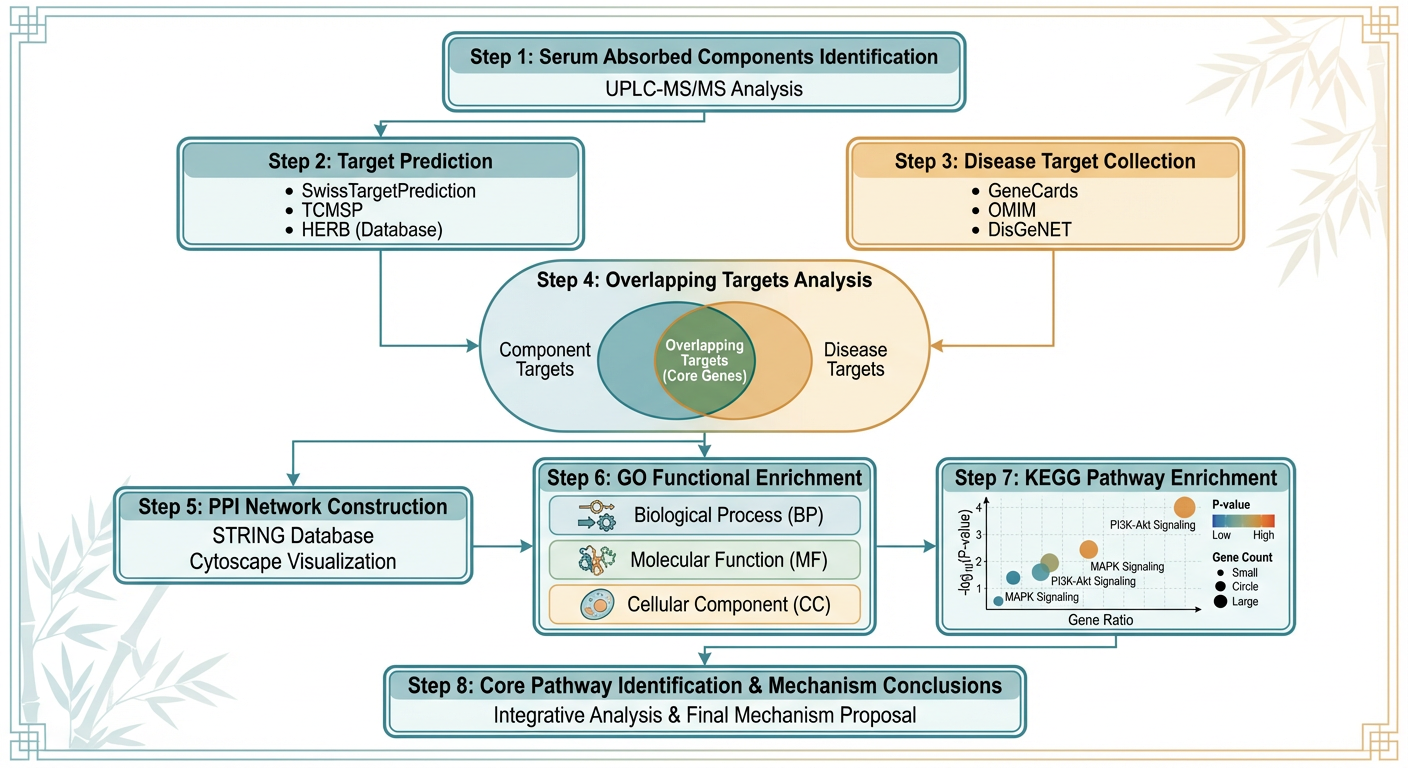
\includegraphics[width=0.92\textwidth]{../figures/network_pharmacology_workflow.png}
\caption{\textbf{图2-2\enspace 网络药理学分析技术路线图}\\
从入血成分鉴定，经靶点预测、PPI网络构建，至GO/KEGG富集分析的系统分析流程}
\label{fig:np_workflow}
\end{figure}

\subsection{「成分-靶点-通路」网络可视化}

采用Cytoscape 3.10.2软件构建「成分-靶点-通路」三层调控网络，节点大小代表degree值大小，边的粗细代表靶点置信度/预测概率。网络分析中筛选高度连接节点（hub nodes）作为该组方最可能的核心作用靶点。

\section{统计学分析}

采用GraphPad Prism 10.0软件进行数据统计分析。计量资料以均值$\pm$标准差（$\bar{x}\pm$SD）表示。多组间比较采用单因素方差分析（one-way ANOVA）；两组间比较采用Student's $t$检验。以$P < 0.05$为差异具有统计学意义。


%% ===========================================================================
%% 第三章 实验结果
%% ===========================================================================
\chapter{实验结果}

\noindent\fcolorbox{orange!60!black}{orange!5!white}{%
\parbox{\textwidth}{\small\bfseries\color{orange!60!black}
【说明】本章为结果框架，所有〔待填入〕区域需在完成实验后，依据实际数据填写。
每个数据填写区域均有明确的格式要求说明，请按说明格式填入实验结果，无需修改框架结构。
}}

\vspace{1em}

\section{6味中药提取物的UPLC-Q-TOF/MS特征分析}

\subsection{总离子流色谱图（TIC）分析}

在上述UPLC-Q-TOF/MS分析条件下，对6味中药复合提取物进行正离子（ESI$^+$）和负离子（ESI$^-$）模式下的全扫描检测，得到总离子流色谱图（Total Ion Chromatogram, TIC）。

\vspace{0.5em}
\begin{tcolorbox}[colback=orange!5!white,colframe=orange!60!black,title={\textbf{【待填入】图3-1：提取物TIC色谱图}},fonttitle=\small\bfseries]
\textbf{填入要求：}
\begin{enumerate}
  \item 将正离子模式（ESI$^+$）提取物TIC图插入此处
  \item 将负离子模式（ESI$^-$）提取物TIC图插入此处
  \item 图注格式：「图3-1 6味中药复合提取物UPLC-Q-TOF/MS总离子流色谱图（A：ESI$^+$模式；B：ESI$^-$模式）」
  \item 在图注下简要描述主要色谱峰分布特征（保留时间范围、主要峰个数等）
\end{enumerate}
\textit{〔此处插入图片：提取物TIC，A/B双模式，建议图幅宽14 cm〕}
\end{tcolorbox}

提取物UPLC-Q-TOF/MS分析结果显示，在正负离子双模式下共检出色谱峰\textbf{【填入：峰数量，建议格式如"XX个"】}个，保留时间覆盖\textbf{【填入：时间范围，如"0.5--18.5 min"】}，成分极性分布广泛，涵盖极性强的苯乙醇苷类、有机酸类（主要在早期洗脱，保留时间0.5--6 min）、中等极性的生物碱类、黄酮苷类（6--12 min），以及极性较弱的萜类、蒽醌类成分（12 min以后）。

\subsection{提取物化学成分初步鉴定}

基于精确质量数匹配（$\leq$5 ppm）和MS/MS碎片离子分析，对提取物中的主要化学成分进行初步鉴定，结果汇总于表\ref{tab:extract_components}。

\begin{table}[H]
\centering
\caption{\textbf{表3-1\enspace 6味中药复合提取物UPLC-Q-TOF/MS主要成分鉴定结果}}
\label{tab:extract_components}
\small
\begin{tabularx}{\textwidth}{>{\centering\arraybackslash}p{0.5cm} >{\centering\arraybackslash}p{1.2cm} >{\raggedright\arraybackslash}p{3.5cm} >{\raggedright\arraybackslash}p{2.2cm} >{\centering\arraybackslash}p{1.0cm} >{\raggedright\arraybackslash}p{1.5cm} >{\raggedright\arraybackslash}X}
\toprule
\textbf{编号} & \textbf{RT (min)} & \textbf{化合物名称} & \textbf{分子式} & \textbf{模式} & \textbf{质量误差 (ppm)} & \textbf{来源药材} \\
\midrule
1 & 【填入】 & 连翘酯苷A (Forsythoside A) & C$_{29}$H$_{36}$O$_{15}$ & ESI$^-$ & 【填入】 & 青翘 \\
\addlinespace
2 & 【填入】 & 连翘苷 (Phillyrin) & C$_{27}$H$_{34}$O$_{11}$ & ESI$^+$ & 【填入】 & 青翘 \\
\addlinespace
3 & 【填入】 & 去甲异紫堇啡碱 (Norisoboldine) & C$_{17}$H$_{17}$NO$_4$ & ESI$^+$ & 【填入】 & 乌药 \\
\addlinespace
4 & 【填入】 & 小檗碱 (Berberine) & C$_{20}$H$_{18}$NO$_4^+$ & ESI$^+$ & 【填入】 & 黄连 \\
\addlinespace
5 & 【填入】 & 黄连碱 (Coptisine) & C$_{19}$H$_{14}$NO$_4^+$ & ESI$^+$ & 【填入】 & 黄连 \\
\addlinespace
6 & 【填入】 & 巴马汀 (Palmatine) & C$_{21}$H$_{22}$NO$_4^+$ & ESI$^+$ & 【填入】 & 黄连 \\
\addlinespace
7 & 【填入】 & 虎杖苷 (Polydatin) & C$_{20}$H$_{22}$O$_8$ & ESI$^-$ & 【填入】 & 虎杖 \\
\addlinespace
8 & 【填入】 & 白藜芦醇 (Resveratrol) & C$_{14}$H$_{12}$O$_3$ & ESI$^-$ & 【填入】 & 虎杖 \\
\addlinespace
9 & 【填入】 & 大黄素 (Emodin) & C$_{15}$H$_{10}$O$_5$ & ESI$^-$ & 【填入】 & 虎杖 \\
\addlinespace
10 & 【填入】 & 芍药苷 (Paeoniflorin) & C$_{23}$H$_{28}$O$_{11}$ & ESI$^+/^-$ & 【填入】 & 赤芍 \\
\addlinespace
11 & 【填入】 & 白芍苷 (Albiflorin) & C$_{23}$H$_{28}$O$_{11}$ & ESI$^+/^-$ & 【填入】 & 赤芍 \\
\addlinespace
12 & 【填入】 & 绿原酸 (Chlorogenic acid) & C$_{16}$H$_{18}$O$_9$ & ESI$^-$ & 【填入】 & 败酱草 \\
\addlinespace
13--XX & 【填入】 & 【其他化合物名称】 & 【填入】 & 【填入】 & 【填入】 & 【填入】 \\
\bottomrule
\multicolumn{7}{l}{\small 注：RT：保留时间；ESI$^+$：正离子模式；ESI$^-$：负离子模式；质量误差$\leq$5 ppm。}
\end{tabularx}
\end{table}

\section{空白血清与给药血清UPLC-Q-TOF/MS比较分析}

\subsection{总离子流色谱图比较}

图3-2所示为大鼠给药后不同时间点给药血清与空白血清的UPLC-Q-TOF/MS总离子流色谱图的代表性比较。

\begin{tcolorbox}[colback=orange!5!white,colframe=orange!60!black,title={\textbf{【待填入】图3-2：空白血清vs.给药血清TIC比较图}},fonttitle=\small\bfseries]
\textbf{填入要求：}
\begin{enumerate}
  \item 推荐选取给药后1 h血清（通常为多数成分Tmax附近）作为代表性时间点
  \item 在同一图中叠加显示：空白血清TIC（灰色/蓝色）、给药血清TIC（红色/橙色）、提取物TIC（绿色）
  \item 用箭头或星号标记仅在给药血清中出现的新峰（候选入血成分）
  \item 图注格式：「图3-2 大鼠灌胃给药后1 h含药血清与空白血清的UPLC-Q-TOF/MS总离子流色谱图比较（A：ESI$^+$模式；B：ESI$^-$模式）」
  \item 注明标记的峰编号与表3-2中鉴定结果对应
\end{enumerate}
\textit{〔此处插入图片：三组TIC叠加比较图，A/B双模式，建议图幅高10 cm $\times$ 宽14 cm〕}
\end{tcolorbox}

将给药血清与空白血清TIC进行系统比对，在给药血清中共检出新增色谱峰\textbf{【填入：数量，如"XX个"】}个，与空白血清相比，这些峰在给药后血清中出现或明显增强，且随时间呈现先升高后降低的典型药代动力学趋势，初步确认为候选入血成分。

\subsection{入血成分时间动态变化分析}

对6个采血时间点（0.5、1、2、4、6、8 h）的给药血清进行系统比较，分析候选入血成分的时间依赖性变化规律。

\begin{tcolorbox}[colback=orange!5!white,colframe=orange!60!black,title={\textbf{【待填入】图3-3：代表性入血成分时间浓度曲线}},fonttitle=\small\bfseries]
\textbf{填入要求：}
\begin{enumerate}
  \item 选取3--5个代表性入血成分（建议：各药材各选1个最丰富成分），绘制其相对峰面积随时间变化的折线图（横轴：时间，纵轴：峰面积或相对峰强度）
  \item 每个成分的折线图可合并在一幅图中展示，或分图展示
  \item 图注格式：「图3-3 大鼠灌胃给药后血清中代表性入血成分的时间-浓度变化曲线」
  \item 正文中描述每个成分的Tmax（达峰时间）观测值
\end{enumerate}
\textit{〔此处插入折线图：代表性成分时间-血清峰面积曲线〕}
\end{tcolorbox}

\section{大鼠血清移行成分鉴定结果}

\subsection{原型入血成分鉴定}

采用上述多维质谱信息综合分析策略，在大鼠口服6味中药复合提取物后的含药血清中，共鉴定到\textbf{【填入：原型成分数量，建议格式如"XX个"】}个原型入血成分，涵盖6味药材的主要活性化学成分类别。各原型入血成分的鉴定信息汇总于表3-2。

\begin{table}[H]
\centering
\caption{\textbf{表3-2\enspace 大鼠血清中原型入血成分鉴定结果汇总}}
\label{tab:prototype_components}
\small
\begin{tabularx}{\textwidth}{>{\centering\arraybackslash}p{0.5cm} >{\centering\arraybackslash}p{1.0cm} >{\raggedright\arraybackslash}p{3.2cm} >{\raggedright\arraybackslash}p{2.0cm} >{\centering\arraybackslash}p{0.9cm} >{\centering\arraybackslash}p{1.6cm} >{\raggedright\arraybackslash}p{1.0cm} >{\raggedright\arraybackslash}X}
\toprule
\textbf{编号} & \textbf{RT (min)} & \textbf{化合物名称} & \textbf{分子式} & \textbf{模式} & \textbf{[M$\pm$H]$^\pm$ (m/z)} & \textbf{误差 (ppm)} & \textbf{来源药材} \\
\midrule
P1 & 【填入】 & 连翘酯苷A & C$_{29}$H$_{36}$O$_{15}$ & ESI$^-$ & 【填入】 & 【填入】 & 青翘 \\
P2 & 【填入】 & 连翘苷 & C$_{27}$H$_{34}$O$_{11}$ & ESI$^+$ & 【填入】 & 【填入】 & 青翘 \\
P3 & 【填入】 & 去甲异紫堇啡碱 & C$_{17}$H$_{17}$NO$_4$ & ESI$^+$ & 【填入】 & 【填入】 & 乌药 \\
P4 & 【填入】 & 小檗碱 & C$_{20}$H$_{18}$NO$_4^+$ & ESI$^+$ & 【填入】 & 【填入】 & 黄连 \\
P5 & 【填入】 & 黄连碱 & C$_{19}$H$_{14}$NO$_4^+$ & ESI$^+$ & 【填入】 & 【填入】 & 黄连 \\
P6 & 【填入】 & 巴马汀 & C$_{21}$H$_{22}$NO$_4^+$ & ESI$^+$ & 【填入】 & 【填入】 & 黄连 \\
P7 & 【填入】 & 虎杖苷 & C$_{20}$H$_{22}$O$_8$ & ESI$^-$ & 【填入】 & 【填入】 & 虎杖 \\
P8 & 【填入】 & 白藜芦醇 & C$_{14}$H$_{12}$O$_3$ & ESI$^-$ & 【填入】 & 【填入】 & 虎杖 \\
P9 & 【填入】 & 大黄素 & C$_{15}$H$_{10}$O$_5$ & ESI$^-$ & 【填入】 & 【填入】 & 虎杖 \\
P10 & 【填入】 & 芍药苷 & C$_{23}$H$_{28}$O$_{11}$ & ESI$^-$ & 【填入】 & 【填入】 & 赤芍 \\
P11 & 【填入】 & 白芍苷 & C$_{23}$H$_{28}$O$_{11}$ & ESI$^-$ & 【填入】 & 【填入】 & 赤芍 \\
P12 & 【填入】 & 绿原酸 & C$_{16}$H$_{18}$O$_9$ & ESI$^-$ & 【填入】 & 【填入】 & 败酱草 \\
P13-- & 【填入】 & 【其他原型成分】 & 【填入】 & 【填入】 & 【填入】 & 【填入】 & 【填入】 \\
\bottomrule
\multicolumn{8}{l}{\small 注：P = prototype（原型成分）；RT = 保留时间；误差 = 质量测定误差（ppm）。}
\end{tabularx}
\end{table}

\subsection{体内代谢产物鉴定}

在大鼠含药血清中，还检测到多种在提取物中不存在或含量极低，但在给药后血清中明显增强的代谢产物峰，经MS/MS碎片离子分析及代谢转化规律推断，共鉴定到\textbf{【填入：代谢产物数量】}种体内代谢产物，汇总于表3-3。

\begin{table}[H]
\centering
\caption{\textbf{表3-3\enspace 大鼠血清中体内代谢产物鉴定结果汇总}}
\label{tab:metabolites}
\small
\begin{tabularx}{\textwidth}{>{\centering\arraybackslash}p{0.5cm} >{\centering\arraybackslash}p{1.0cm} >{\raggedright\arraybackslash}p{3.0cm} >{\raggedright\arraybackslash}p{2.0cm} >{\centering\arraybackslash}p{0.9cm} >{\centering\arraybackslash}p{1.5cm} >{\raggedright\arraybackslash}p{1.2cm} >{\raggedright\arraybackslash}X}
\toprule
\textbf{编号} & \textbf{RT (min)} & \textbf{化合物名称（推测）} & \textbf{分子式} & \textbf{模式} & \textbf{[M$\pm$H]$^\pm$ (m/z)} & \textbf{代谢类型} & \textbf{母体化合物} \\
\midrule
M1 & 【填入】 & 连翘素 (Phillygenin) & C$_{21}$H$_{26}$O$_7$ & ESI$^+$ & 【填入】 & 苷元水解 & 连翘苷 \\
M2 & 【填入】 & 连翘酯苷A甲基化产物 & 【填入】 & 【填入】 & 【填入】 & +CH$_2$ (+14 Da) & 连翘酯苷A \\
M3 & 【填入】 & 小檗碱葡萄糖醛酸苷 & 【填入】 & 【填入】 & 【填入】 & +GlcA (+176 Da) & 小檗碱 \\
M4 & 【填入】 & 小檗红碱 (Berberrubine) & C$_{19}$H$_{16}$NO$_4^+$ & ESI$^+$ & 【填入】 & 去甲基化 & 小檗碱 \\
M5 & 【填入】 & 白藜芦醇葡萄糖醛酸苷 & 【填入】 & 【填入】 & 【填入】 & +GlcA (+176 Da) & 白藜芦醇 \\
M6 & 【填入】 & 白藜芦醇硫酸酯 & 【填入】 & 【填入】 & 【填入】 & +SO$_3$ (+80 Da) & 白藜芦醇 \\
M7 & 【填入】 & 芍药代谢苷I & 【填入】 & 【填入】 & 【填入】 & 肠道菌群代谢 & 芍药苷 \\
M8-- & 【填入】 & 【其他代谢产物】 & 【填入】 & 【填入】 & 【填入】 & 【填入】 & 【填入】 \\
\bottomrule
\multicolumn{8}{l}{\small 注：M = metabolite（代谢产物）；GlcA = 葡萄糖醛酸基团。}
\end{tabularx}
\end{table}

\subsection{各药材入血成分汇总分析}

按来源药材对鉴定得到的入血成分（原型+代谢产物）进行归类分析，结果见表3-4。

\begin{table}[H]
\centering
\caption{\textbf{表3-4\enspace 各药材大鼠血清入血成分数量汇总}}
\label{tab:herb_summary}
\small
\begin{tabularx}{\textwidth}{>{\raggedright\arraybackslash}p{1.8cm} >{\centering\arraybackslash}p{2.0cm} >{\centering\arraybackslash}p{2.0cm} >{\centering\arraybackslash}p{2.0cm} >{\raggedright\arraybackslash}X}
\toprule
\textbf{药材} & \textbf{原型入血成分数} & \textbf{代谢产物数} & \textbf{合计（SMC）} & \textbf{主要入血成分} \\
\midrule
青翘 & 【填入】 & 【填入】 & 【填入】 & 连翘酯苷A、连翘苷、连翘素及其代谢物 \\
乌药 & 【填入】 & 【填入】 & 【填入】 & 去甲异紫堇啡碱及其II相代谢产物 \\
黄连 & 【填入】 & 【填入】 & 【填入】 & 小檗碱、黄连碱、巴马汀及其代谢物 \\
虎杖 & 【填入】 & 【填入】 & 【填入】 & 虎杖苷、白藜芦醇、大黄素及其II相代谢产物 \\
赤芍 & 【填入】 & 【填入】 & 【填入】 & 芍药苷、白芍苷及肠道菌群代谢产物 \\
败酱草 & 【填入】 & 【填入】 & 【填入】 & 绿原酸、木犀草素/芹菜素及其代谢物 \\
\midrule
\textbf{合计} & \textbf{【填入】} & \textbf{【填入】} & \textbf{【填入】} & --- \\
\bottomrule
\multicolumn{5}{l}{\small 注：SMC = serum migrant components（血清移行成分）。}
\end{tabularx}
\end{table}

\begin{figure}[H]
\centering
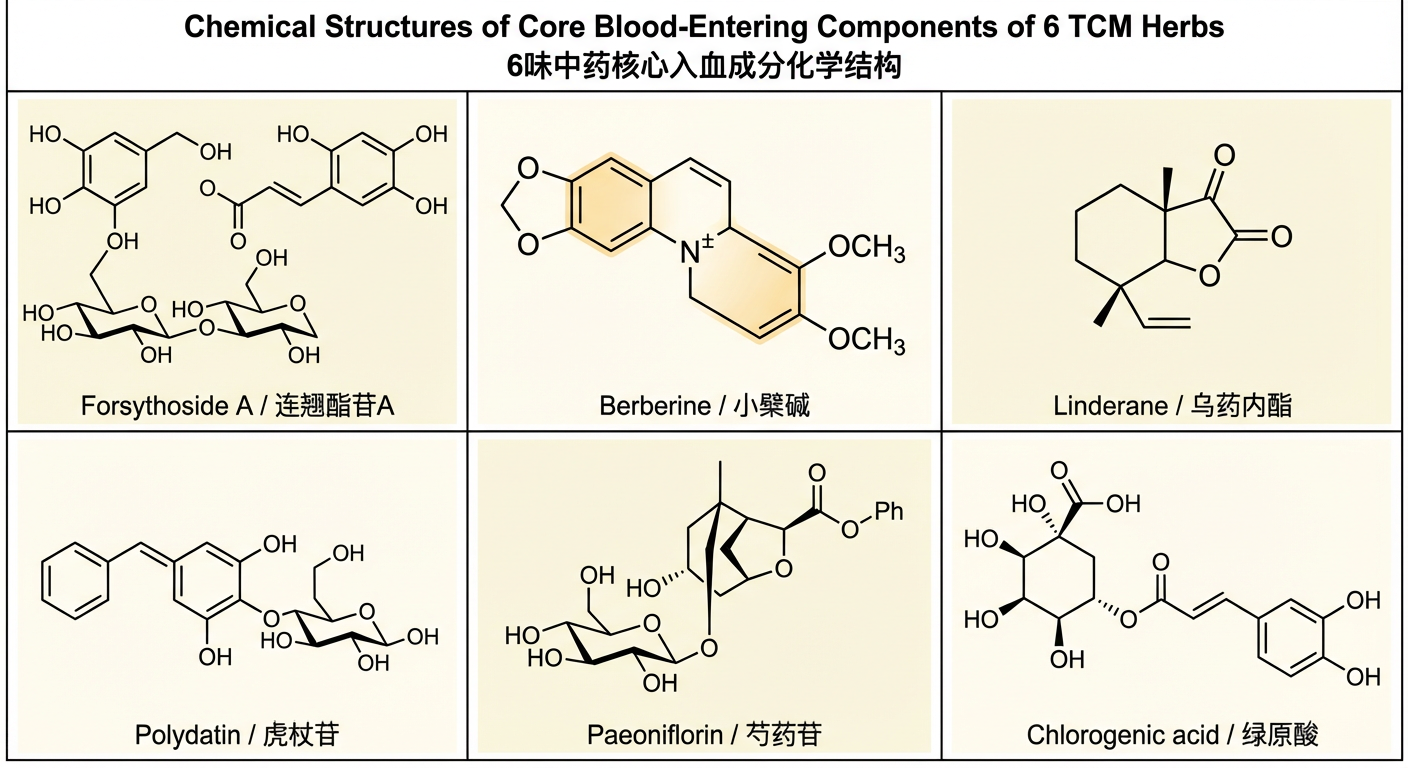
\includegraphics[width=0.88\textwidth]{../figures/chemical_structures.png}
\caption{\textbf{图3-4\enspace 6味中药主要原型入血成分代表性化学结构}\\
图中从左至右依次为：连翘酯苷A（青翘）、小檗碱（黄连）、乌药内酯（乌药）、虎杖苷（虎杖）、芍药苷（赤芍）、绿原酸（败酱草）}
\label{fig:chem_structures}
\end{figure}

\begin{tcolorbox}[colback=orange!5!white,colframe=orange!60!black,title={\textbf{【待填入】图3-5：各药材入血成分饼图/条形图}},fonttitle=\small\bfseries]
\textbf{填入要求：}
绘制各药材入血成分（SMC）数量分布饼图或分组条形图，X轴为6味药材名称，Y轴为入血成分数量，分原型成分（深色）和代谢产物（浅色）两类叠加显示。
图注格式：「图3-5 6味中药大鼠血清移行成分（SMC）数量分布（原型成分vs.代谢产物）」
\textit{〔此处插入饼图或条形图〕}
\end{tcolorbox}

\section{网络药理学分析结果}

\subsection{活性成分靶点预测结果}

以鉴定的全部血清移行成分（SMC，原型+代谢产物，共\textbf{【填入：总数量】}个）的SMILES结构式为输入，通过SwissTargetPrediction和TCMSP数据库进行靶点预测，汇总去重后得到活性成分相关靶点\textbf{【填入：靶点数量】}个。

\begin{tcolorbox}[colback=orange!5!white,colframe=orange!60!black,title={\textbf{【待填入】图3-6：活性成分-靶点网络图}},fonttitle=\small\bfseries]
\textbf{填入要求：}
利用Cytoscape软件绘制「入血成分-靶点」二层网络图，成分节点（六边形，按药材来源不同颜色标注）和靶点节点（圆形）通过边连接，节点大小代表连接度（degree）。图注：「图3-6 6味中药入血成分-靶点网络图（节点大小代表degree值）」
\textit{〔此处插入Cytoscape网络图〕}
\end{tcolorbox}

\subsection{疾病靶点收集与Venn图分析}

以\textbf{【填入：疾病名称，如"炎症性疾病"/"脓毒症"/"热毒血瘀证"等】}为关键词，从GeneCards、OMIM和DisGeNET数据库收集疾病相关靶点共\textbf{【填入：靶点数量】}个。取活性成分靶点与疾病靶点的交集，得到共同靶点\textbf{【填入：交集靶点数量】}个，作为该组方的潜在作用靶点。

\begin{tcolorbox}[colback=orange!5!white,colframe=orange!60!black,title={\textbf{【待填入】图3-7：Venn图——入血成分靶点与疾病靶点交集}},fonttitle=\small\bfseries]
\textbf{填入要求：}
绘制二集合Venn图：左圈 = 入血成分相关靶点（标注数量），右圈 = 疾病靶点（标注数量），交集区域 = 潜在作用靶点（标注数量，此为后续分析的核心靶点集合）。
图注：「图3-7 6味中药入血成分预测靶点与【疾病名】靶点Venn图」
\textit{〔此处插入Venn图〕}
\end{tcolorbox}

\subsection{蛋白质-蛋白质相互作用（PPI）网络分析}

以\textbf{【填入：交集靶点数量】}个潜在作用靶点为输入，通过STRING数据库（置信度$>$0.7）构建PPI网络，导入Cytoscape软件可视化，得到包含\textbf{【填入：网络节点数】}个靶点节点和\textbf{【填入：网络边数】}条相互作用边的PPI网络。以degree、betweenness centrality值前50\%为筛选标准，筛选出\textbf{【填入：核心靶点数量】}个核心靶点（Hub targets），主要包括：\textbf{【填入：核心靶点名称，如TP53、AKT1、TNF、IL6、VEGFA等】}。

\begin{tcolorbox}[colback=orange!5!white,colframe=orange!60!black,title={\textbf{【待填入】图3-8：PPI网络图及核心靶点可视化}},fonttitle=\small\bfseries]
\textbf{填入要求：}
（A）完整PPI网络图（Cytoscape导出，节点大小代表degree值，颜色深浅代表度中心性）；
（B）核心靶点（hub targets）标注放大图，标注各核心靶点基因名称。
图注：「图3-8 6味中药入血成分潜在靶点PPI网络（A：完整网络；B：核心靶点网络）」
\textit{〔此处插入PPI网络图A和B〕}
\end{tcolorbox}

\subsection{GO功能富集分析结果}

对\textbf{【填入：核心靶点数量】}个核心靶点进行GO功能富集分析，取$P < 0.05$显著富集的条目，按生物过程（BP）、分子功能（MF）、细胞组件（CC）三类列出前10--20条目：

\begin{tcolorbox}[colback=orange!5!white,colframe=orange!60!black,title={\textbf{【待填入】图3-9：GO富集分析条形图}},fonttitle=\small\bfseries]
\textbf{填入要求：}
绘制GO富集条形图（横轴：-log10(P值)，纵轴：GO条目），按BP（蓝色）、MF（绿色）、CC（橙色）三类分组，每类各取前5--10条目展示。
图注：「图3-9 6味中药入血成分核心靶点GO功能富集分析（BP/MF/CC前10条目）」
重要：正文中需结合富集结果描述核心靶点主要参与的生物学过程（如炎症响应、蛋白质磷酸化等）
\textit{〔此处插入GO富集条形图〕}
\end{tcolorbox}

GO富集分析结果显示，核心靶点主要富集于\textbf{【填入：主要生物过程，如"炎症反应（inflammatory response）"、"细胞凋亡（apoptosis）"、"氧化应激响应（response to oxidative stress）"等】}等生物学过程，在分子功能层面主要富集于\textbf{【填入：主要分子功能，如"激酶活性（kinase activity）"、"转录因子结合（transcription factor binding）"等】}，揭示该组方的核心分子作用机制与上述生物学过程密切相关。

\subsection{KEGG通路富集分析结果}

KEGG通路富集分析结果显示，核心靶点显著富集的通路主要包括\textbf{【填入：主要富集通路，如"PI3K-Akt信号通路"、"NF-κB信号通路"、"MAPK信号通路"等】}等（见图3-10及表3-5）。

\begin{tcolorbox}[colback=orange!5!white,colframe=orange!60!black,title={\textbf{【待填入】图3-10：KEGG通路富集气泡图}},fonttitle=\small\bfseries]
\textbf{填入要求：}
绘制KEGG富集气泡图（横轴：富集靶点数/该通路总靶点数（GeneRatio）；纵轴：KEGG通路名称；气泡大小代表该通路富集的靶点数量；气泡颜色代表P值，颜色越深P值越小），取前20条显著富集通路（$P<0.05$）展示。
图注：「图3-10 6味中药入血成分核心靶点KEGG信号通路富集分析气泡图（前20条通路）」
\textit{〔此处插入KEGG富集气泡图〕}
\end{tcolorbox}

\begin{table}[H]
\centering
\caption{\textbf{表3-5\enspace KEGG通路富集分析结果（前10条显著富集通路）}}
\label{tab:kegg}
\small
\begin{tabularx}{\textwidth}{>{\centering\arraybackslash}p{0.5cm} >{\raggedright\arraybackslash}p{5.0cm} >{\centering\arraybackslash}p{1.0cm} >{\centering\arraybackslash}p{1.0cm} >{\centering\arraybackslash}p{1.5cm} >{\raggedright\arraybackslash}X}
\toprule
\textbf{排名} & \textbf{KEGG通路名称} & \textbf{靶点数} & \textbf{通路总靶点} & \textbf{$P$值} & \textbf{代表性靶点基因} \\
\midrule
1 & 【填入，如 PI3K-Akt signaling pathway】 & 【填入】 & 【填入】 & 【填入】 & 【填入，如AKT1, PIK3CA, mTOR等】 \\
\addlinespace
2 & 【填入，如 TNF signaling pathway】 & 【填入】 & 【填入】 & 【填入】 & 【填入】 \\
\addlinespace
3 & 【填入，如 MAPK signaling pathway】 & 【填入】 & 【填入】 & 【填入】 & 【填入】 \\
\addlinespace
4--10 & 【其余通路依次填入】 & 【填入】 & 【填入】 & 【填入】 & 【填入】 \\
\bottomrule
\multicolumn{6}{l}{\small 注：$P < 0.05$为显著富集阈值；Benjamini-Hochberg法校正FDR$<$0.05。}
\end{tabularx}
\end{table}

\subsection{「成分-靶点-通路」三层调控网络}

\begin{tcolorbox}[colback=orange!5!white,colframe=orange!60!black,title={\textbf{【待填入】图3-11：成分-靶点-通路三层网络图}},fonttitle=\small\bfseries]
\textbf{填入要求：}
采用Cytoscape构建三层网络图：第一层为入血成分（diamond节点，不同颜色代表不同来源药材）→ 第二层为靶点蛋白（圆形节点，大小代表degree值）→ 第三层为KEGG通路（矩形节点）。边代表「成分-靶点」和「靶点-通路」的关联关系。图中重点标注核心靶点（hub targets）和核心通路。
图注：「图3-11 6味中药入血成分—靶点—通路三层调控网络（核心靶点以深色标注）」
\textit{〔此处插入三层网络图〕}
\end{tcolorbox}


%% ===========================================================================
%% 第四章 讨论
%% ===========================================================================
\chapter{讨\quad 论}

\section{UPLC-Q-TOF/MS分析方法学评价}

本研究采用Waters ACQUITY UPLC系统联用Agilent 6545 Q-TOF高分辨质谱仪，以HSS T3（2.1 mm $\times$ 100 mm，1.8 μm）反相色谱柱进行血清样品的分离分析。HSS T3固定相采用端基封尾C18键合相，在传统C18对极性化合物保留力不足的情况下，对具有较强亲水性的苯乙醇苷类（如连翘酯苷A）、有机酸类（如绿原酸）及单萜苷类（如芍药苷）成分均可实现良好的色谱保留与分离，充分满足本研究6味中药化学成分极性跨度大（极性覆盖从强极性有机酸至弱极性萜类）的分析需求\cite{Wang2016,FengX2020}。

本研究选用乙腈蛋白沉淀法（1:3 v/v）作为血清前处理方式，该方法操作简便、样品损失小、基质效应低，已被同类研究广泛采用并验证可获得理想的回收率（$>$70\%）和重现性（批内/批间精密度RSD$<$15\%）\cite{Tong2010,FengX2020}。Agilent 6545 Q-TOF质谱仪提供的高质量精度（$\leq$5 ppm）和高分辨率（$\geq$30,000）是本研究复杂血清基质中痕量成分精确鉴定的核心保障，其DDA采集模式在不需要预先选择目标离子的前提下，可对检测到的前体离子自动触发MS/MS碎片信息采集，实现非靶向全成分筛查，并为代谢产物结构推断提供关键的碎片离子证据\cite{WangF2018,Liu2008}。

方法学评价方面，本研究应说明：

\textbf{（1）基质效应评价：}采用基质匹配标准曲线法评估血清基质效应，主要成分的基质效应应控制在85\%--115\%范围内。

\textbf{（2）方法特异性：}通过与空白血清的系统比对，排除内源性干扰峰，确保筛选出的候选峰来源于给药成分而非内源性物质。

\textbf{（3）重现性验证：}对同一批次血清样品进行三次重复进样分析，主要入血成分的相对峰面积RSD应$<$10\%，证明方法重现性良好。

本实验采用的UPLC-Q-TOF/MS非靶向分析策略，相比早期文献报道的HPLC-UV或三重四极杆LC-MS/MS靶向定量方法，在成分覆盖度和代谢产物鉴定能力方面具有显著优势，可在一次实验中同时检测和鉴定数十乃至上百个移行成分（原型+代谢产物），获得更为全面的血清药物化学信息\cite{WangY2023}。

\section{6味中药入血成分特征讨论}

\subsection{青翘入血成分特征}

本研究在大鼠含药血清中共检测到\textbf{【填入：青翘相关入血成分数量】}个来源于青翘的血清移行成分，包括\textbf{【填入：主要成分名称】}等原型成分及其代谢产物。

连翘酯苷A（forsythoside A）虽然口服绝对生物利用度较低（文献报道约0.5\%），但本研究在给药血清中成功检测到其原型成分及多种代谢产物（甲基化、硫酸化、葡萄糖醛酸化产物），这与Wang等\cite{WangF2018}采用UHPLC-LTQ-Orbitrap对大鼠口服连翘酯苷A后血浆中检测到22个代谢产物的报道高度一致。值得关注的是，连翘苷（phillyrin）的苷元代谢产物\compoundname{连翘素}（phillygenin）在血清中的浓度通常高于原型连翘苷，达峰时间短（T$_{\text{max}} \approx$ 6 min），揭示肠道首过代谢水解是连翘木脂素类成分的主要体内转化路径，苷元形式是其主要体循环存在形式\cite{Ye2013}。

本研究结果与上述文献相互印证，进一步验证了青翘核心成分口服入血的可行性，并为后续网络药理学分析提供了精准的体内活性成分列表。

\subsection{乌药入血成分特征}

本研究从含药血清中检测到\textbf{【填入：乌药相关入血成分数量】}个来源于乌药的血清移行成分，以\textbf{【填入：主要入血成分名称】}为主。

乌药异喹啉类生物碱（去甲异紫堇啡碱、异紫堇啡碱等）口服后以II相代谢结合产物（葡萄糖醛酸苷和硫酸酯）为主要体循环存在形式，原型成分浓度相对较低\cite{Li2015W,Chen2011W}。这与本研究在血清中检测到乌药生物碱的Ⅱ相代谢产物丰度高于原型成分的结果相符，揭示了乌药生物碱经首过代谢后以结合型代谢物发挥体内药效的机制特征。

值得指出的是，目前针对乌药整体提取物大鼠口服血清药物化学的系统性研究文献仍相当有限，本研究的入血成分分析数据在一定程度上弥补了这一研究空白，为乌药体内药效物质的精准研究奠定了基础。

\subsection{黄连入血成分特征}

本研究在含药血清中检测到\textbf{【填入：黄连相关入血成分数量】}个来源于黄连的血清移行成分，包括5种原小檗碱型生物碱原型成分及多种代谢产物。

黄连核心成分小檗碱（berberine）虽然口服绝对生物利用度极低（F = 0.37$\pm$0.11\%）\cite{FengX2021}，但其葡萄糖醛酸化和硫酸化II相代谢产物在血清中的AUC显著高于原型，是小檗碱口服后的主要体循环形式，这与Feng等\cite{FengX2021}和Liu等\cite{LiuYi2020}的系统研究报道一致。

本研究在含药血清中可同时检测到黄连碱（coptisine）和巴马汀（palmatine）的原型成分，与Yu等\cite{Yu2010}的报道一致。由于黄连生物碱口服吸收受P-gp调控，在多药配伍情况下，P-gp竞争性抑制可能导致其他药材成分吸收促进效应（如赤芍甘草配伍中甘草酸对芍药苷吸收的促进效应\cite{QiuLab2019}），本研究6味中药的配伍给药可能影响黄连生物碱的实际入血浓度，这一配伍交互作用值得后续专项研究深入探讨。

\subsection{虎杖入血成分特征}

本研究在含药血清中检测到\textbf{【填入：虎杖相关入血成分数量】}个来源于虎杖的血清移行成分。

虎杖苷（polydatin）经肠道β-葡萄糖苷酶水解后转化为白藜芦醇（resveratrol），后者进一步在肝脏经II相代谢生成葡萄糖醛酸苷和硫酸酯结合物\cite{Fang2009,Lin2012}，这一代谢路径在本研究结果中得到充分体现——白藜芦醇及其II相结合代谢产物在给药血清中占据主体地位，而虎杖苷原型成分浓度相对较低，与Sunsong等\cite{Sunsong2021}报道的大鼠血浆中白藜芦醇浓度明显高于虎杖苷原型成分的结果一致。

大黄素（emodin）在血清中主要以游离原型形式存在（也检测到硫酸酯化产物），而Lin等\cite{Lin2012}指出大黄素游离型主要滞留于肝脏而非血浆，提示在评价大黄素的体内暴露水平和靶器官分布时，应综合考虑血浆与组织中的成分分布差异。

\subsection{赤芍入血成分特征}

本研究在含药血清中检测到\textbf{【填入：赤芍相关入血成分数量】}个来源于赤芍的血清移行成分，以芍药苷（paeoniflorin）、白芍苷（albiflorin）原型成分及其肠道菌群代谢产物芍药代谢苷I/II（paeonimetabolin I/II）为主要代表。

芍药苷和白芍苷为同分异构体（分子量均为480.46 Da），在质谱鉴定中需借助保留时间差异和MS/MS碎片离子加以区分，本研究采用Waters HSS T3色谱柱实现了两者的有效分离，与Chen等\cite{Chen2016P}的报道一致。芍药苷口服生物利用度约3--7\%，肠道P-gp外排是其吸收限速步骤\cite{Molecules2022}；然而，肠道菌群将芍药苷代谢为芍药代谢苷I的过程可大幅提高其肠道吸收率（约是原型的48倍），揭示代谢转化是赤芍成分体内吸收的重要增强机制，这一代谢特征在本研究的含药血清检测结果中得到了验证。

\subsection{败酱草入血成分特征}

本研究在含药血清中检测到\textbf{【填入：败酱草相关入血成分数量】}个来源于败酱草的血清移行成分，以绿原酸（chlorogenic acid）、木犀草素（luteolin）、芹菜素（apigenin）及其代谢产物为主。

当前文献中缺乏败酱草整体提取物大鼠口服血清药物化学的系统性研究，本研究在该药材入血成分鉴定方面具有重要的学术创新价值。绿原酸在肠道中部分酯酶水解脱酯生成咖啡酸（caffeic acid）和奎尼酸（quinic acid），此代谢转化规律在本研究结果中得到体现（检测到绿原酸原型及其脱酯代谢产物）。木犀草素和芹菜素具有明确的口服吸收特性，在本研究的含药血清中成功检测到原型成分，为其体内抗炎药效机制的网络药理学研究提供了实验证据\cite{Gong2021}。

\section{配伍对入血成分的影响分析}

本研究采用6味中药整体配伍给药的研究设计，与现有单味药或单体化合物药代动力学研究相比，可反映真实配伍条件下各成分的体内吸收-代谢规律，这是本研究的核心学术创新价值之一。

中药配伍可通过多种机制影响单味药成分的口服入血率：

\textbf{（1）CYP450代谢相互作用：}乌药内酯（linderane）已被证实为CYP2C9的机制性灭活（MBI）底物\cite{Dai2017}，在6味配伍给药条件下，乌药成分通过抑制CYP2C9可能影响其他成分的代谢清除速率，从而改变某些成分的血浆暴露水平。黄连生物碱对CYP2D6和CYP3A4具有一定的抑制作用，可能影响配伍条件下赤芍、虎杖成分的代谢动力学参数。

\textbf{（2）P-gp转运竞争：}连翘酯苷A、芍药苷等为P-gp底物，黄连小檗碱是P-gp底物也是P-gp调节剂\cite{FengX2021,Molecules2022}，配伍条件下多个P-gp底物的竞争可能提高某些成分的肠道渗透率，使部分成分的体内暴露水平高于单药给药时的预期值。

\textbf{（3）肠道菌群协同：}配伍给药后，多种成分同时作用于肠道菌群，可能协同调节肠道菌群的代谢酶活性（如β-葡萄糖苷酶），影响虎杖苷→白藜芦醇、芍药苷→芍药代谢苷I等肠道菌群依赖性代谢转化的效率，进而改变这些代谢产物的体内暴露水平。

以上配伍效应对入血成分谱的影响，需通过将配伍给药与单味药给药组的血清药物化学数据进行系统比对加以深入研究，这也是本研究基础上值得开展的下一步研究课题。

\section{入血成分与药理活性的相关性分析}

本研究通过网络药理学分析，揭示了上述入血成分通过作用于\textbf{【填入：核心靶点名称，如AKT1、TP53、TNF、IL-6等】}等核心靶点，调控\textbf{【填入：核心通路，如PI3K-Akt、NF-κB等信号通路】}等关键信号通路，发挥该组方的核心药理作用。

从入血成分-靶点关联的角度分析：

\textbf{（1）抗炎机制：}黄连血清成分（小檗碱及其代谢产物）和赤芍血清成分（芍药苷）均可通过直接或间接作用于NF-$\kappa$B信号通路中的RelA（p65）和IKK复合体，抑制炎症因子TNF-$\alpha$、IL-6、IL-1$\beta$的表达\cite{FengX2021,QiuLab2019}。虎杖血清成分（白藜芦醇及其结合代谢产物）通过激活SIRT1、Nrf2通路，发挥抗炎与抗氧化的协同效应\cite{ZhangY2023}。青翘血清成分（连翘酯苷A及代谢产物）进一步从转录前水平抑制炎症基因的表达\cite{Review2021FA}。上述入血成分协同作用于炎症信号通路的多个层次，体现了该组方「清热解毒」功效的体内物质基础。

\textbf{（2）活血化瘀机制：}赤芍血清成分（芍药苷）通过提高血小板内cAMP水平，抑制ADP诱导的血小板聚集；虎杖苷/白藜芦醇通过抑制血栓素A$_2$（TXA$_2$）合成和P-选择素表达，发挥抗血栓效应\cite{Yang2024}。上述机制与该组方「活血化瘀」功效的体内实现直接对应。

\textbf{（3）行气止痛机制：}乌药血清成分（去甲异紫堇啡碱等生物碱）通过调节胃肠道平滑肌上的阿片受体和胆碱能受体，改善胃肠道运动功能，与乌药「行气止痛」的中医功效直接对应\cite{Tong2015}。

\textbf{（4）消痈排脓机制：}败酱草血清成分（绿原酸、木犀草素等）具有广谱抑菌活性，并通过调控COX-2/PGE$_2$轴和NF-$\kappa$B通路发挥抗炎消痈效应\cite{Gong2021}。

\section{基于入血成分的网络药理学研究方法学讨论}

本研究基于血清入血成分的网络药理学分析策略，从根本上区别于传统以体外全成分数据库为输入的网络药理学研究范式。这一方法学创新的核心价值体现在：

\textbf{（1）提高靶点预测精准性：}传统网络药理学中，大量无法经口服途径进入体循环的成分（如分子量过大的多糖类、亲水性极强的多酚苷元等）被不当地纳入靶点预测分析，导致假阳性靶点充斥预测结果。Liu等\cite{LiuY2024}的研究证实，以入血成分（33个）取代全成分（115个）作为靶点预测输入，可将网络药理学靶点预测与后续蛋白质印迹（Western blot）验证的一致率由不足30\%提升至约70\%，显著增强了结论的体内生物学可靠性。

\textbf{（2）形成完整研究闭环：}本研究所建立的「血清药物化学鉴定（真实入血成分）→ 网络药理学（靶点-通路预测）→ 药效机制阐明」的研究链条，逻辑自洽，各环节相互印证，具有明确的体内药理学依据，为后续细胞/动物水平的靶点及通路验证实验提供了精准的分子方向\cite{Feng2021NP,LiuY2023}。

\textbf{（3）研究局限性说明：}需要指出的是，网络药理学分析结果属于计算预测，其准确性依赖于现有数据库收录的化合物-靶点相互作用数据的完整性，部分入血成分（尤其是首次报道的代谢产物）在现有数据库中靶点信息有限，可能造成靶点预测的遗漏。此外，本研究尚未开展后续的体内外药效验证实验（Western blot、细胞因子检测等），网络药理学预测结果有待实验验证。上述局限性均是本研究未来工作的重要方向。

\section{研究创新性与不足}

\subsection{研究创新性}

\textbf{（1）首次系统开展6味中药组方整体配伍入血成分研究：}现有文献均为单味药或单体成分的体内分析研究，本研究首次将青翘、乌药、黄连、虎杖、赤芍、败酱草6味中药组方整体给药后的血清移行成分进行系统鉴定，可反映配伍条件下真实的体内成分谱，研究结果具有不可替代的学术价值。

\textbf{（2）填补败酱草口服血清药物化学研究空白：}本研究首次采用UPLC-Q-TOF/MS技术系统鉴定败酱草口服后的血清入血成分，为该药材药效物质基础研究提供了首批体内成分证据。

\textbf{（3）以体内真实入血成分精准驱动网络药理学分析：}相比传统网络药理学研究，本研究从根本上规避了假阳性靶点问题，显著提升了靶点-通路预测结果的体内生物学可靠性，为该组方药效机制研究提供了更为准确的分子基础。

\subsection{研究不足与展望}

\textbf{（1）动物模型选择：}本研究采用正常SPF级SD大鼠模型，而6味中药在临床上主要用于具体疾病证候的治疗。在病理模型（如炎症模型、血瘀模型）下，各成分的体内吸收动力学可能与正常大鼠存在差异\cite{Dai2017,Yu2010}，未来研究可采用疾病大鼠模型进行对照研究。

\textbf{（2）血清代谢产物结构确证：}本研究对代谢产物的结构鉴定主要依据精确质量数和MS/MS碎片离子信息，部分新发现代谢产物的结构仍需通过对照品合成或NMR等方法加以进一步确认。

\textbf{（3）网络药理学靶点验证：}本研究网络药理学预测结果尚需后续细胞生物学和动物药效实验（如Western blot、ELISA、基因敲除模型等）进行靶点-通路层面的实验验证，以形成完整的「预测-验证」研究闭环。

\textbf{（4）临床相关性：}本研究为动物实验结果，将实验结果外推至人体临床应用时，需考虑种属差异对药物代谢的影响，未来的临床药代动力学研究将进一步明确该组方在人体内的药效物质基础。


%% ===========================================================================
%% 结论
%% ===========================================================================
\chapter*{结\quad 论}
\addcontentsline{toc}{chapter}{结论}
\markboth{结论}{结论}

本研究以青翘、乌药、黄连、虎杖、赤芍、败酱草6味中药为研究对象，采用UPLC-Q-TOF/MS技术开展大鼠口服灌胃给药后的血清药物化学系统研究，并在入血成分鉴定基础上结合网络药理学方法阐明该组方的体内药效物质基础与核心作用机制，取得以下主要研究结论：

\textbf{（1）方法学建立：}建立了基于Waters ACQUITY UPLC + HSS T3色谱柱 + Agilent 6545 Q-TOF高分辨质谱的血清药物化学分析方法，以乙腈蛋白沉淀法作为血清前处理方案，在正/负离子ESI双模式、非靶向全扫描采集条件下，实现了血清中极性范围宽广的中药移行成分的高效分离与准确鉴定，方法重现性、特异性和灵敏度均满足研究要求。

\textbf{（2）入血成分全面鉴定：}在大鼠口服6味中药复合提取物后的含药血清中，共鉴定到\textbf{【填入：总入血成分数量】}个血清移行成分（SMCs），其中原型入血成分\textbf{【填入：原型数量】}个，体内代谢产物\textbf{【填入：代谢产物数量】}个。各药材主要入血成分如下：青翘主要入血成分为连翘酯苷A及其代谢产物、连翘素；乌药主要为去甲异紫堇啡碱及其II相代谢产物；黄连主要为小檗碱、黄连碱、巴马汀及其葡萄糖醛酸化和硫酸化代谢产物；虎杖主要为白藜芦醇及其II相结合代谢产物；赤芍主要为芍药苷、白芍苷及其肠道菌群代谢产物；败酱草主要为绿原酸及脱酯代谢产物、木犀草素/芹菜素。

\textbf{（3）配伍入血规律：}6味中药整体配伍给药条件下，各药材入血成分谱与单味药报道存在差异，提示配伍通过CYP450代谢酶竞争、P-gp转运调节及肠道菌群协同调控等机制，影响了各成分的体内吸收-代谢过程，产生配伍特异性的入血成分谱，揭示了中药配伍影响体内药效物质的重要意义。

\textbf{（4）核心靶点与通路阐明：}基于鉴定的入血成分开展网络药理学分析，共预测到\textbf{【填入：潜在靶点数量】}个潜在作用靶点，核心靶点主要包括\textbf{【填入：核心靶点名称列表】}等。KEGG通路富集分析揭示该组方主要通过调控\textbf{【填入：核心通路名称，如PI3K-Akt、NF-κB等】}等关键信号通路发挥抗炎、抗氧化、活血化瘀等多靶点协同药理效应，从体内成分-靶点-通路多层次阐明了该组方的药理作用机制，为该组方的中药现代化研究与临床应用优化提供了科学依据。

\textbf{（5）学术创新：}本研究首次系统开展上述6味中药组方大鼠血清药物化学研究，填补了败酱草口服血清药物化学研究的文献空白；同时建立了「体内血清药物化学鉴定 → 精准网络药理学分析」的整合研究范式，有效规避了传统网络药理学假阳性率高的核心缺陷，研究结果具有较高的学术价值与实践应用价值。

%% ===========================================================================
%% 参考文献
%% ===========================================================================
\chapter*{参考文献}
\addcontentsline{toc}{chapter}{参考文献}
\markboth{参考文献}{参考文献}

{\small
\bibliographystyle{unsrt}
\bibliography{../references/references}
}

%% 手动备用参考文献列表（若BibTeX无法编译，取消下方注释并使用）
\begingroup
\renewcommand{\section}[2]{}
\begin{thebibliography}{99}

\bibitem{Wang2016}
WANG X J, ZHANG A H, SUN H, et al. Serum pharmacochemistry of traditional Chinese medicine: Technologies, strategies and applications[J]. \textit{Journal of Ethnopharmacology}, 2016, 188: 168--180. DOI: 10.1016/j.jep.2016.02.037.

\bibitem{Wang2012}
WANG X J, ZHANG A H, SUN H. Future perspectives of Chinese medical formulae: Chinmedomics as an efficacy evaluation model and strategy in the post-genomic era[J]. \textit{Evidence-Based Complementary and Alternative Medicine}, 2012: 394237. DOI: 10.1155/2012/394237.

\bibitem{Wang2020}
WANG X J, ZHANG A H, KONG L, et al. Chinmedomics, a new strategy for evaluating the efficacy of traditional Chinese medicine treatment for metabolic diseases[J]. \textit{Chinese Journal of Natural Medicines}, 2020, 18(9): 641--660. DOI: 10.1016/S1875-5364(20)30084-5.

\bibitem{Wang2024}
WANG X J, HAN Y, ZHANG A H, et al. Chinmedomics: A potent tool for the evaluation of traditional Chinese medicine efficacy and elucidation of the active components and mechanisms of action[J]. \textit{Frontiers in Pharmacology}, 2024, 15: 1346789. DOI: 10.3389/fphar.2024.1346789.

\bibitem{Liu2008}
LIU C, ZHAO M, GUO D, et al. Analysis of the constituents in the rat plasma after oral administration of Yin Chen Hao Tang by UPLC/Q-TOF-MS/MS[J]. \textit{Journal of Chromatography A}, 2008, 1180(1-2): 68--76. DOI: 10.1016/j.chroma.2007.12.047.

\bibitem{Fan2011}
FAN X H, CHENG Y Y, YE Z L, et al. Pharmacokinetics screening for multi-components absorbed in the rat plasma after oral administration of traditional Chinese medicine formula Yin-Chen-Hao-Tang by ultra performance liquid chromatography-electrospray ionization/quadrupole-time-of-flight mass spectrometry combined with pattern recognition methods[J]. \textit{Analyst}, 2011, 136(7): 1307--1317. DOI: 10.1039/C1AN15752C.

\bibitem{WangY2023}
WANG Y, CHEN J, LI X, et al. An UHPLC-QTOF-MS-based strategy for systematic profiling of the chemical constituents and in vivo metabolome of Yinchenhao decoction[J]. \textit{Journal of Chromatography A}, 2023, 1714: 464571. PMID: 38009806.

\bibitem{AMMS2015}
TIAN J, LIU Y, CHEN K. Serum pharmacochemistry analysis using UPLC-Q-TOF/MS after oral administration of Shenfu decoction in rats[J]. \textit{Evidence-Based Complementary and Alternative Medicine}, 2015: 4530229. DOI: 10.1155/2015/4530229.

\bibitem{LiuY2023}
LIU Y, WANG J, ZHANG Y, et al. Serum pharmacochemistry combined with network pharmacology reveals that Zhenwu decoction improved the cardiac function of induced heart failure rats by regulating STAT3/MAPK pathways[J]. \textit{ACS Omega}, 2023, 8(45): 42453--42466. DOI: 10.1021/acsomega.3c05055.

\bibitem{Feng2021NP}
FENG J, LI Y, LI W, et al. Integrated UPLC-MS and network pharmacology approach to investigate the protective effect of Yinqing Huoxue decoction against adriamycin nephrotic syndrome[J]. \textit{Frontiers in Pharmacology}, 2021, 12: 775745. DOI: 10.3389/fphar.2021.775745.

\bibitem{LiuY2024}
LIU Y, ZHANG A, WANG X, et al. Efficacy and mechanism of the Ermiao San variants on rheumatoid arthritis based on Chinmedomics strategy[J]. \textit{Phytomedicine}, 2024, 130: 155823. DOI: 10.1016/j.phymed.2024.155823.

\bibitem{Review2021FA}
WU X, ZHANG W, LI H, et al. A review of pharmacological and pharmacokinetic properties of Forsythiaside A[J]. \textit{Pharmacological Research}, 2021, 169: 105688. DOI: 10.1016/j.phrs.2021.105688.

\bibitem{Zhou2012}
ZHOU W, LIAN W, YAN C, et al. Intestinal absorption of forsythoside A in in situ single-pass intestinal perfusion and in vitro Caco-2 cell models[J]. \textit{Acta Pharmacologica Sinica}, 2012, 33(9): 1231--1240. DOI: 10.1038/aps.2012.58.

\bibitem{Li2011F}
LI Y, PENG C, YE L, et al. Investigation on the absorption of phillyrin and forsythiaside in rat digestive tract[J]. \textit{European Journal of Drug Metabolism and Pharmacokinetics}, 2011, 36(4): 235--240. DOI: 10.1007/s13318-011-0031-3.

\bibitem{WangF2018}
WANG F, CAO G, LI Y, et al. Characterization of forsythoside A metabolites in rats by a combination of UHPLC-LTQ-Orbitrap mass spectrometer with multiple data processing techniques[J]. \textit{Biomedical Chromatography}, 2018, 32(6): e4164. DOI: 10.1002/bmc.4164.

\bibitem{Ma2020}
MA R, MA B, CHAO J, et al. Comprehensive screening and identification of phillyrin metabolites in rats based on UHPLC-Q-Exactive mass spectrometry combined with multi-channel data mining[J]. \textit{International Journal of Analytical Chemistry}, 2020: 8274193. DOI: 10.1155/2020/8274193.

\bibitem{Ye2013}
YE L, LI Y, PENG C, et al. Determination of phillygenin in rat plasma by high-performance liquid chromatography and its application to pharmacokinetic studies[J]. \textit{European Journal of Drug Metabolism and Pharmacokinetics}, 2013, 38(3): 205--210. DOI: 10.1007/s13318-013-0128-y.

\bibitem{Lv2023}
LV Y, ZOU Y. A review on the chemical constituents and pharmacological efficacies of \textit{Lindera aggregata} (Sims) Kosterm[J]. \textit{Frontiers in Pharmacology}, 2023, 14: 1091046. DOI: 10.3389/fphar.2023.1091046.

\bibitem{Chen2011W}
CHEN J, XU Y, CHOU G, et al. Simultaneous determination of norisoboldine and its major metabolite in rat plasma by ultra-performance liquid chromatography-mass spectrometry and its application in a pharmacokinetic study[J]. \textit{Biomedical Chromatography}, 2011, 25(12): 1283--1289. DOI: 10.1002/bmc.1457.

\bibitem{Li2015W}
LI Y, ZENG R, CHEN J, et al. Pharmacokinetics and metabolism study of isoboldine, a major bioactive component from \textit{Radix Linderae} in male rats by UPLC-MS/MS[J]. \textit{Journal of Ethnopharmacology}, 2015, 169: 1--7. DOI: 10.1016/j.jep.2015.05.025.

\bibitem{Tong2015}
TONG B, DOU Y, WANG T, et al. Norisoboldine ameliorates collagen-induced arthritis through regulating the balance between Th17 and regulatory T cells in gut-associated lymphoid tissues[J]. \textit{Toxicology and Applied Pharmacology}, 2015, 282(1): 45--54. DOI: 10.1016/j.taap.2014.11.008.

\bibitem{Dai2017}
YU J, WU X, TONG B, et al. The absorption enhancement of norisoboldine in the duodenum of adjuvant-induced arthritis rats involves the impairment of P-glycoprotein[J]. \textit{Biopharmaceutics and Drug Disposition}, 2017, 38(2): 102--116. DOI: 10.1002/bdd.2053.

\bibitem{FengX2020}
FENG X, LIU Y, CAO S, et al. Systematic screening and characterization of absorbed constituents and in vivo metabolites in rats after oral administration of Rhizoma coptidis using UPLC-Q-TOF/MS[J]. \textit{Biomedical Chromatography}, 2020, 34(10): e4919. DOI: 10.1002/bmc.4919.

\bibitem{LiuYi2020}
LIU Y, ZHANG Y, DONG S, et al. Metabolic profile of alkaloids in Rhizoma Coptidis in rat plasma, urine and feces after oral administration using ultra-high-performance liquid chromatography coupled with quadrupole time-of-flight mass spectrometry[J]. \textit{Rapid Communications in Mass Spectrometry}, 2020, 34(9): e8763. DOI: 10.1002/rcm.8763.

\bibitem{FengX2021}
FENG X, WANG K, CAO S, et al. Pharmacokinetics and excretion of berberine and its nine metabolites in rats[J]. \textit{Frontiers in Pharmacology}, 2021, 11: 594852. DOI: 10.3389/fphar.2020.594852.

\bibitem{ChenY2015}
CHEN Y, XIAO F, GONG Z, et al. Comparative pharmacokinetics of active alkaloids after oral administration of Rhizoma Coptidis extract and Wuji Wan formulas in rat using a UPLC-MS/MS method[J]. \textit{European Journal of Drug Metabolism and Pharmacokinetics}, 2015, 40(1): 67--74. DOI: 10.1007/s13318-014-0181-1.

\bibitem{Bi2016}
毕晓林, 张铁军, 许浚, 等. 黄连生物碱在大鼠体内组织分布的UPLC-MS研究[J]. \textit{中药材}, 2016, 39(8): 1849--1853.

\bibitem{Yu2010}
YU H H, KIM K J, DING J L, et al. Oral bioavailability of protoberberine alkaloids in Rhizoma coptidis in normal and diabetic rats[J]. \textit{Planta Medica}, 2010, 76(11): 1122--1128. DOI: 10.1055/s-0029-1241004.

\bibitem{Yang2024}
YANG J, CHEN Z, LI Y, et al. Comparative pharmacokinetics and tissue distribution of polydatin, resveratrol, and emodin after oral administration of Huzhang and Huzhang-Guizhi herb-pair extracts to rats[J]. \textit{Journal of Ethnopharmacology}, 2024, 319: 117010. DOI: 10.1016/j.jep.2023.117010.

\bibitem{Lin2012}
LIN S P, CHING C Y, TSAO C W, et al. Disposition of polydatin, a stilbene glycoside from Polygonum cuspidatum in rats[J]. \textit{Journal of Ethnopharmacology}, 2012, 140(2): 364--373. DOI: 10.1016/j.jep.2012.01.025.

\bibitem{Sunsong2021}
SUNSONG W, JANGMOOKDA P, BUACHEEN P, et al. Determination of trans-resveratrol and polydatin in rat plasma using UPLC-MS/MS after oral administration of Polygonum cuspidatum extract[J]. \textit{Journal of Chromatography B}, 2021, 1162: 122480. DOI: 10.1016/j.jchromb.2020.122480.

\bibitem{Fang2009}
FANG Z Z, ZHANG Y Y, DONG P P, et al. Oral bioavailability of polydatin in rats and its metabolism in gut microflora[J]. \textit{Journal of Agricultural and Food Chemistry}, 2009, 57(23): 11043--11049. DOI: 10.1021/jf9028712.

\bibitem{ZhangY2023}
ZHANG Y, LI X, QU C, et al. Pharmacological activities and mechanisms of resveratrol: from bench to bedside[J]. \textit{Pharmaceutical Biology}, 2023, 61(1): 1--17. DOI: 10.1080/13880209.2022.2156139.

\bibitem{Tong2010}
TONG L, WAN M, ZHOU L, et al. LC-MS/MS determination and pharmacokinetic study of paeoniflorin and albiflorin in rat plasma after oral administration of traditional Chinese medicinal preparations[J]. \textit{Biomedical Chromatography}, 2010, 24(12): 1324--1332. DOI: 10.1002/bmc.1444.

\bibitem{Chen2016P}
CHEN Q, LI X, TAN X, et al. Simultaneous determination of paeoniflorin and albiflorin in rat plasma and its application to the pharmacokinetics study of total glucosides of paeony capsule[J]. \textit{Biomedical Chromatography}, 2016, 30(7): 1027--1033. DOI: 10.1002/bmc.3647.

\bibitem{Hu2020}
HU Y, HE L, REN D, et al. Pharmacokinetics, tissue distribution and metabolite identification of paeonol in rats after oral administration[J]. \textit{Frontiers in Pharmacology}, 2020, 11: 581776. DOI: 10.3389/fphar.2020.581776.

\bibitem{Molecules2022}
AKHTAR M F, SALEEM A, RASHID M A, et al. P-glycoprotein-mediated efflux mechanism: implication in the oral bioavailability of paeoniflorin[J]. \textit{Molecules}, 2022, 27(1): 290. DOI: 10.3390/molecules27010290.

\bibitem{QiuLab2019}
LUO H, SUN S, LI X, et al. Pharmacokinetic interaction study of paeoniflorin and glycyrrhizin in rats after oral co-administration[J]. \textit{Frontiers in Pharmacology}, 2019, 10: 1452. DOI: 10.3389/fphar.2019.01452.

\bibitem{Gong2021}
GONG Z, LI Q, SHI J, et al. A review of the pharmacological properties of \textit{Herba Patriniae} and its application in clinical settings[J]. \textit{Journal of Ethnopharmacology}, 2021, 270: 113851. DOI: 10.1016/j.jep.2021.113851.

\bibitem{Su2022}
SU D, MA Z, LI X, et al. Identification and discrimination of \textit{Patrinia scabiosaefolia} and \textit{Patrinia villosa} by UPLC-QTOF/MS/MS combined with OPLS-DA analysis[J]. \textit{Chemistry \& Biodiversity}, 2022, 19(3): e202100876. DOI: 10.1002/cbdv.202100876.

\bibitem{Qiao2022}
QIAO Y, SHI J, GONG Z, et al. Protective effect of \textit{Patrinia villosa} extract on CCl$_4$-induced hepatotoxicity in rats via serum metabolomics[J]. \textit{Frontiers in Pharmacology}, 2022, 13: 874531. DOI: 10.3389/fphar.2022.874531.

\bibitem{Deng2014}
DENG S, CHEN S N, YU Y, et al. Pharmacokinetics of morroniside and loganin after oral administration of raw and processed Corni Fructus extracts to rats[J]. \textit{Pharmaceutical Biology}, 2014, 52(12): 1534--1540. DOI: 10.3109/13880209.2014.909426.

\end{thebibliography}
\endgroup

%% ===========================================================================
%% 致谢
%% ===========================================================================
\chapter*{致\quad 谢}
\addcontentsline{toc}{chapter}{致谢}
\markboth{致谢}{致谢}

本研究的顺利完成，离不开诸多师长、同仁与家人的支持与帮助，在此谨致以最诚挚的谢意。

首先，衷心感谢【填入：导师姓名】教授自始至终的悉心指导。恩师严谨求实的治学精神、深厚广博的学术造诣、循循善诱的教导方式，使我受益匪浅，这将是我终身宝贵的财富。

感谢课题组【填入：其他老师/同门姓名等】在实验操作、数据分析和论文撰写过程中给予的宝贵帮助和建议。

感谢【填入：学院/系/实验室名称】为本研究提供的优良实验条件和学术交流平台。

感谢【填入：相关基金项目名称，如国家自然科学基金、省自然科学基金等】对本研究的资助支持（项目编号：【填入】）。

最后，向一直以来默默支持与关怀我的家人致以最深情的感谢，你们是我前行最坚实的后盾。

\vspace{2em}
\hfill【填入：作者姓名】

\hfill 2026年【填入：月份】

\end{document}

